\documentclass[journal=jacsat,manuscript=article]{achemso}

%%%%%%%%%%%%%%%%%%%%%%%%%%%%%%%%%%%%%%%%%%%%%%%%%%%%%%%%%%%%%%%%%%%%%
%% Place any additional packages needed here.  Only include packages
%% which are essential, to avoid problems later. Do NOT use any
%% packages which require e-TeX (for example etoolbox): the e-TeX
%% extensions are not currently available on the ACS conversion
%% servers.
%%%%%%%%%%%%%%%%%%%%%%%%%%%%%%%%%%%%%%%%%%%%%%%%%%%%%%%%%%%%%%%%%%%%%
\usepackage[version=3]{mhchem} % Formula subscripts using \ce{}
\usepackage{xr}
\usepackage{hyperref}
\hypersetup{
    colorlinks=true,
    linkcolor=blue,
    citecolor=blue,
    filecolor=magenta,      
    urlcolor=blue,
    pdfpagemode=FullScreen,
    }
%%%%%%%%%%%%%%%%%%%%%%%%%%%%%%%%%%%%%%%%%%%%%%%%%%%%%%%%%%%%%%%%%%%%%
%% If issues arise when submitting your manuscript, you may want to
%% un-comment the next line.  This provides information on the
%% version of every file you have used.
%%%%%%%%%%%%%%%%%%%%%%%%%%%%%%%%%%%%%%%%%%%%%%%%%%%%%%%%%%%%%%%%%%%%%
%%\listfiles

%%%%%%%%%%%%%%%%%%%%%%%%%%%%%%%%%%%%%%%%%%%%%%%%%%%%%%%%%%%%%%%%%%%%%
%% Place any additional macros here.  Please use \newcommand* where
%% possible, and avoid layout-changing macros (which are not used
%% when typesetting).
%%%%%%%%%%%%%%%%%%%%%%%%%%%%%%%%%%%%%%%%%%%%%%%%%%%%%%%%%%%%%%%%%%%%%
\newcommand*\mycommand[1]{\texttt{\emph{#1}}}
\newcommand{\bfv}[1]{{\mbox{\boldmath{$#1$}}}}
\newcommand{\x}{\bfv{x}}
%%%%%%%%%%%%%%%%%%%%%%%%%%%%%%%%%%%%%%%%%%%%%%%%%%%%%%%%%%%%%%%%%%%%%
%% Meta-data block
%% ---------------
%% Each author should be given as a separate \author command.
%%
%% Corresponding authors should have an e-mail given after the author
%% name as an \email command. Phone and fax numbers can be given
%% using \phone and \fax, respectively; this information is optional.
%%
%% The affiliation of authors is given after the authors; each
%% \affiliation command applies to all preceding authors not already
%% assigned an affiliation.
%%
%% The affiliation takes an option argument for the short name.  This
%% will typically be something like "University of Somewhere".
%%
%% The \altaffiliation macro should be used for new address, etc.
%% On the other hand, \alsoaffiliation is used on a per author basis
%% when authors are associated with multiple institutions.
%%%%%%%%%%%%%%%%%%%%%%%%%%%%%%%%%%%%%%%%%%%%%%%%%%%%%%%%%%%%%%%%%%%%%
\author{Wei-Tse Hsu}
\author{Pascal T. Merz}
\affiliation{Department of Chemical and Biological Engineering, University of Colorado Boulder, Boulder, CO 80305}
\author{Giovanni Bussi}
\affiliation{Scuola Internazionale Superiore di Studi Avanzati, via Bonomea 265, 34136 Trieste, Italy}
\author{Michael R. Shirts}
\affiliation{Department of Chemical and Biological Engineering, University of Colorado Boulder, Boulder, CO 80305}
\email{michael.shirts@colorado.edu}

%%%%%%%%%%%%%%%%%%%%%%%%%%%%%%%%%%%%%%%%%%%%%%%%%%%%%%%%%%%%%%%%%%%%%
%% The document title should be given as usual. Some journals require
%% a running title from the author: this should be supplied as an
%% optional argument to \title.
%%%%%%%%%%%%%%%%%%%%%%%%%%%%%%%%%%%%%%%%%%%%%%%%%%%%%%%%%%%%%%%%%%%%%
\title
  {Adding alchemical variables to metadynamics to enhance sampling in free energy calculations}

%%%%%%%%%%%%%%%%%%%%%%%%%%%%%%%%%%%%%%%%%%%%%%%%%%%%%%%%%%%%%%%%%%%%%
%% Some journals require a list of abbreviations or keywords to be
%% supplied. These should be set up here, and will be printed after
%% the title and author information, if needed.
%%%%%%%%%%%%%%%%%%%%%%%%%%%%%%%%%%%%%%%%%%%%%%%%%%%%%%%%%%%%%%%%%%%%%
% \abbreviations{IR,NMR,UV}
\keywords{American Chemical Society, \LaTeX}

%%%%%%%%%%%%%%%%%%%%%%%%%%%%%%%%%%%%%%%%%%%%%%%%%%%%%%%%%%%%%%%%%%%%%
%% The manuscript does not need to include \maketitle, which is
%% executed automatically.
%%%%%%%%%%%%%%%%%%%%%%%%%%%%%%%%%%%%%%%%%%%%%%%%%%%%%%%%%%%%%%%%%%%%%
\begin{document}

%%%%%%%%%%%%%%%%%%%%%%%%%%%%%%%%%%%%%%%%%%%%%%%%%%%%%%%%%%%%%%%%%%%%%
%% The "tocentry" environment can be used to create an entry for the
%% graphical table of contents. It is given here as some journals
%% require that it is printed as part of the abstract page. It will
%% be automatically moved as appropriate.
%%%%%%%%%%%%%%%%%%%%%%%%%%%%%%%%%%%%%%%%%%%%%%%%%%%%%%%%%%%%%%%%%%%%%
%\begin{tocentry}

%\end{tocentry}

%%%%%%%%%%%%%%%%%%%%%%%%%%%%%%%%%%%%%%%%%%%%%%%%%%%%%%%%%%%%%%%%%%%%%
%% The abstract environment will automatically gobble the contents
%% if an abstract is not used by the target journal.
%%%%%%%%%%%%%%%%%%%%%%%%%%%%%%%%%%%%%%%%%%%%%%%%%%%%%%%%%%%%%%%%%%%%%
\begin{abstract}
Performing alchemical transformations, in which one molecular system is nonphysically changed to another, is a popular approach adopted in free energy calculations associated with various biophysical processes, such as protein-ligand binding, or the transfer of a molecule between environments. While the sampling of alchemical intermediate states in either parallel (e.g. Hamiltonian replica exchange) or serial manner (e.g. expanded ensemble) can bridge the high-probability regions in the configurational space between two end states of interest, alchemical methods can fail in the scenarios where the most important slow degrees of freedom in the configurational space are almost orthogonal to the alchemical variable, or if the system gets trapped in a deep basin expanding in both the configurational and alchemical space. 

To alleviate these issues, we propose to use alchemical variables as an additional dimension in metadynamics, augmenting the ability both to sample collective variables and to enhance sampling in free energy calculations. In this study, we validate our implementation of ``alchemical metadynamics'' in PLUMED with test systems and alchemical processes with varying complexities and dimensions of collective variable space, including the binding and unbinding of CB8-G3 host-guest binding complex. We show that multi-dimensional alchemical metadynamics can address the challenges mentioned above challenges of traditional alchemical free energy methods and further accelerate sampling by introducing configurational collective variables. The method can trivially be combined with other metadynamics-based algorithms implemented in PLUMED. The necessary PLUMED code changes have already been released for general use in PLUMED 2.8.
\end{abstract}

%%%%%%%%%%%%%%%%%%%%%%%%%%%%%%%%%%%%%%%%%%%%%%%%%%%%%%%%%%%%%%%%%%%%%
%% Start the main part of the manuscript here.
%%%%%%%%%%%%%%%%%%%%%%%%%%%%%%%%%%%%%%%%%%%%%%%%%%%%%%%%%%%%%%%%%%%%%
\section{Introduction}
With the fast advent of high-performance computing (HPC) and parallel computing over the years, molecular simulations such as molecular dynamics (MD) and Monte Carlo (MC) simulations have become increasingly useful in elucidating the dynamics of transformation processes of condensed matter systems. They are most useful when the system can visit all the energetically relevant conformations, in which case we can extract valuable thermodynamic and structural information about the system, such as the solvation free energy of a molecule, or the binding ensemble of a binding complex. However, comprehensive sampling in the phase space is generally challenging in traditional MD simulations because the system must rely on very rare fluctuations to cross the free energy barriers that separate metastable states of interest. This low transition probability between metastable states makes the time scale required for achieving system ergodicity in unbiased sampling impractically long in most systems of interest. 

To address this challenge, a wide variety of advanced sampling methods have been developed in the past decades~\cite{henin2022enhanced}. One particular flavor of advanced sampling methods involves sampling along a set of predefined coarse-grained descriptors of the system, or collective variables (CVs). Traditionally, CVs could be any function of the atomic coordinates of the system, but the optimal ones should correspond to the slowest degrees of freedoms that distinguish different metastable states. Methods relying on the use of CVs include umbrella sampling~\cite{umbrella}, adaptive biasing force~\cite{ABF}, metadynamics~\cite{metad} and their variations~\cite{bussi2006free, bonomi2010enhanced, var2}. 

Another category of advanced sampling methods is known as generalized ensemble algorithms, which includes simulated tempering~\cite{marinari1992simulated}, replica exchange~\cite{TREMD, HREMD}, expanded ensemble~\cite{EXE}, $\lambda$-dynamics~\cite{knight2009lambda}, and their variations~\cite{oshima2019replica, knight2011multisite}. These methods do not require any predefined CVs, but a series of intermediate or auxiliary states with modified probability of the coordinates of the system. These intermediates are chosen to remove or lessen the kinetic barriers between end states of interest. These states are defined by varying the temperature or the Hamiltonian of the system to allow an additional sampling dimension, which created nonphysical pathways for the system to circumvent free energy barriers in the configurational space. Increasing the probability overlap between adjacent intermediate states can often enhance the diffusion in not only the temperature/Hamiltonian direction, but also the configurational space. In replica exchange, these states are sampled with the ensembles progressing forwards in time in parallel, while in serial approaches, a single simulations can move between states in either discrete (expanded ensemble) or continuous space ($\lambda$-dynamics). In order to have even sampling between the states, one must add biases or weights to the higher free energy states so they can be sampled. These weights, which are absent in replica exchange, similarly modify the underlying free energy surface as the biasing potentials in metadynamics do. Notably, these intermediate or auxiliary states can be useful for reasons other than simply accelerating sampling. For example, the sampling in the temperature space allows us to determine thermodynamic observables of interest as a function of temperature, while simulations with alchemical intermediate states are useful for calculating the free energy difference between the end states of alchemical processes. In free energy calculations where the temperature is constant, sampling in alchemical intermediate states obviates the need of defining CVs, which could be non-trivial in systems where the slowest-relaxing coordinates are not intuitive, such as the escape of a ligand from a buried binding pocket~\cite{buried1, buried2}. 

Although sampling in the alchemical variable can create new ensembles where the slowest physical collective variables are not longer so slow, it cannot necessarily enhance sampling where the configurational barriers are almost orthogonal to the alchemical direction. For example, a configurational free energy barrier can be present for all the alchemical states (scenario A in Figure \ref{EXE_issues}) so that the system could remain stuck even if it is able to drift to other alchemical states or cross free energy barriers along the alchemical direction. Another scenario that could easily trap the system is the presence of large free energy basins in both the configurational and alchemical directions (scenario B in Figure \ref{EXE_issues}). In both scenarios, state-dependent weights can only shift the whole free energy profile as a function of relevant configurational CVs with the same amount. They do not change the partition function ratio between points at the same alchemical state but with different values of the configurational CVs, so the sampling in the configurational space can still be limited in these cases.

\begin{figure}[ht]
    \centering
    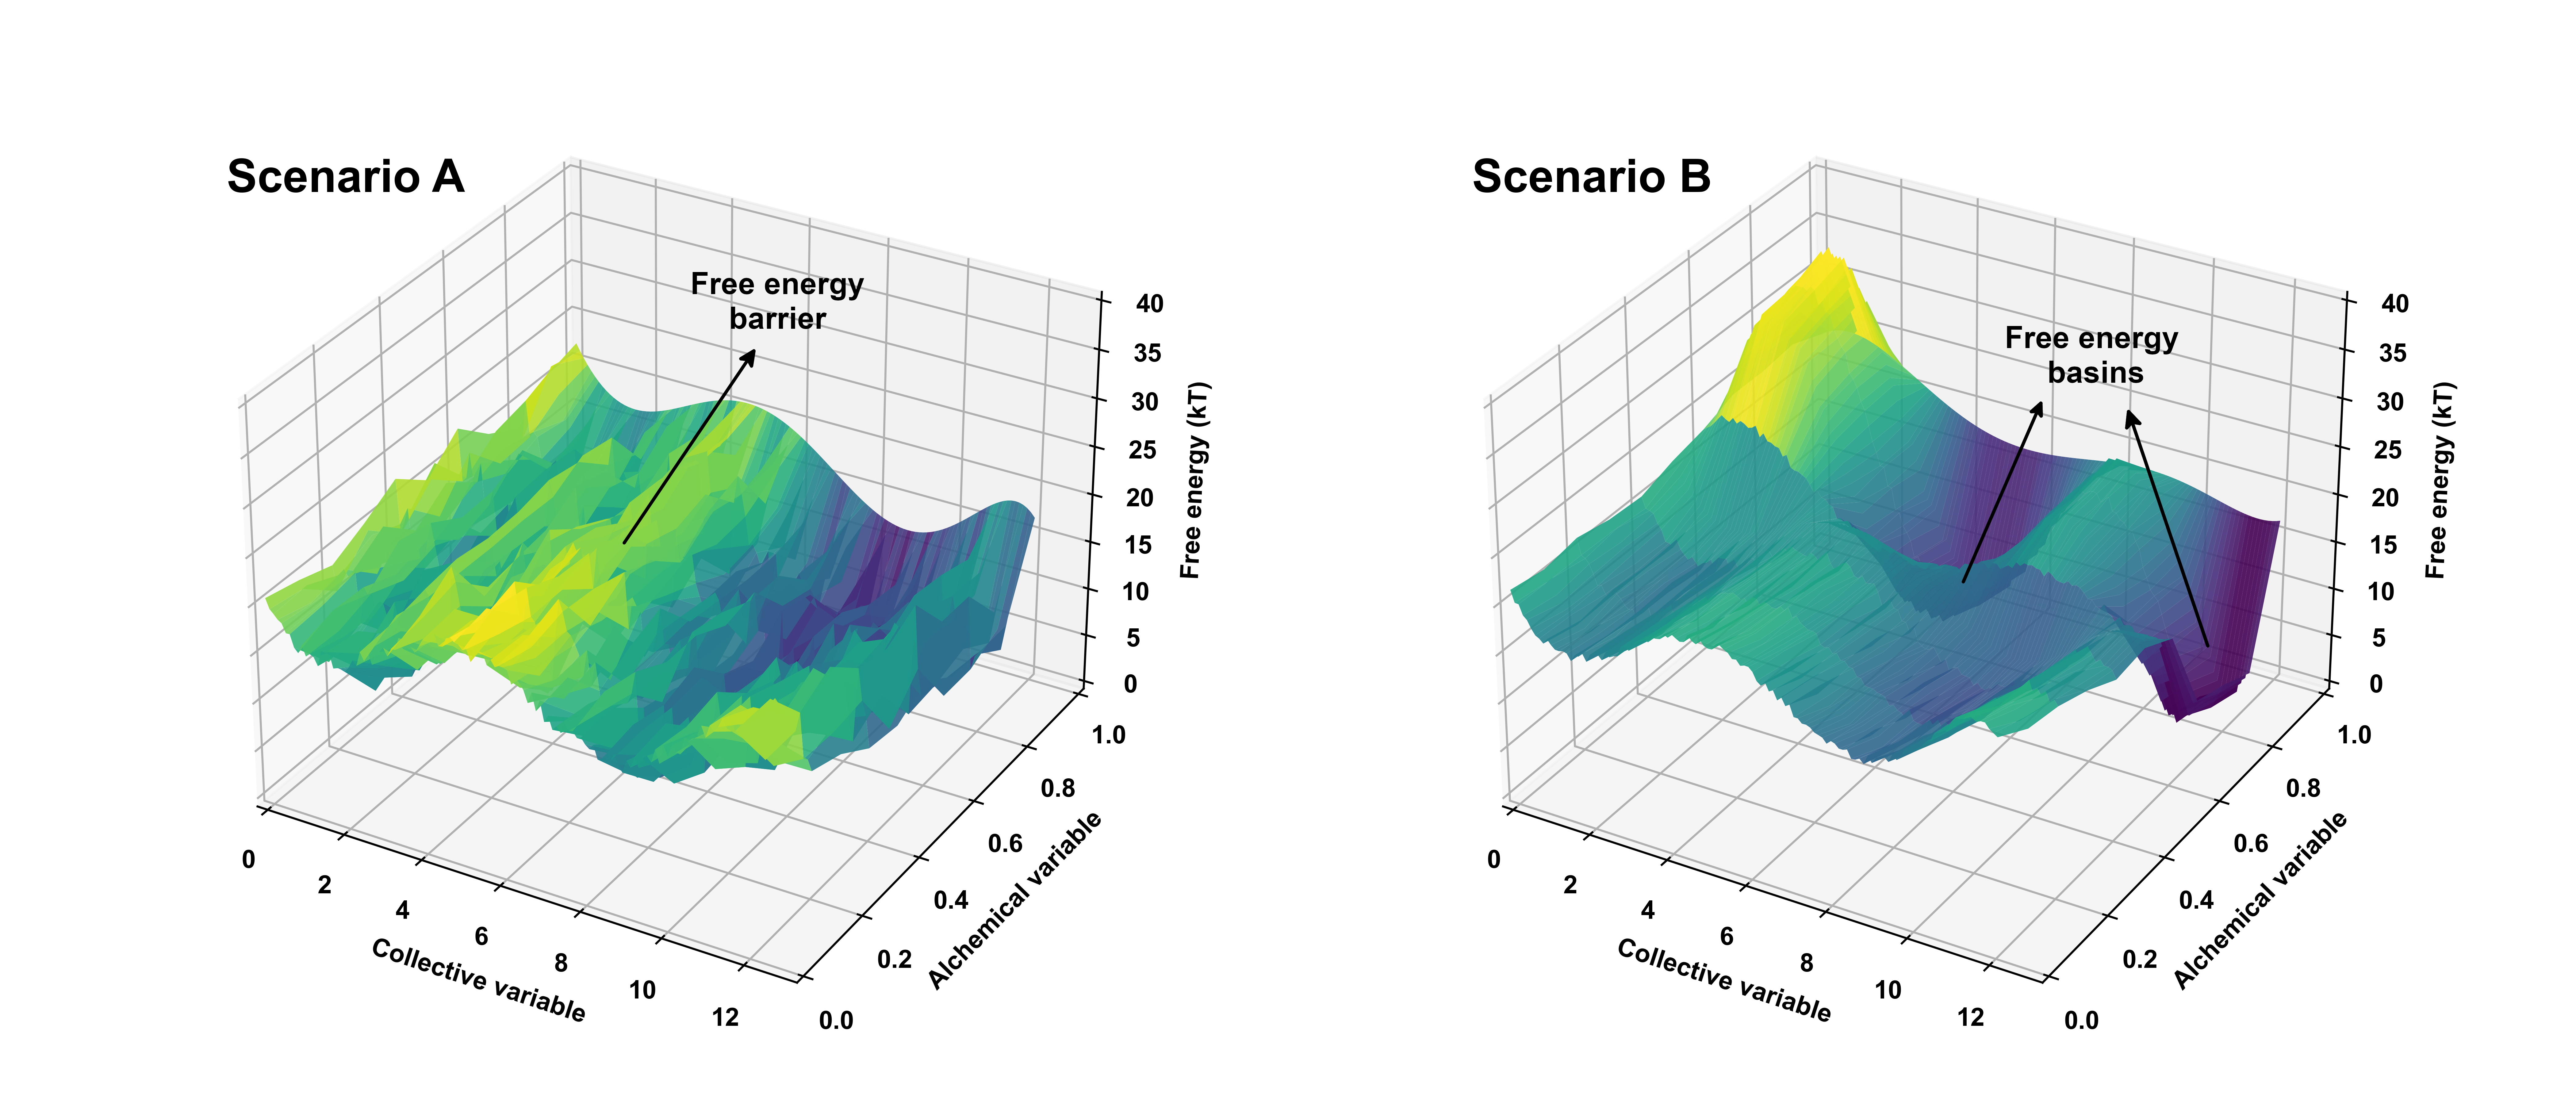
\includegraphics[width=\textwidth]{Figures/EXE_issues_final.png}   
    \caption{Scenarios where pure alchemical bias fails to accelerate configurational sampling. In scenario A, the free energy barrier extending across all $\lambda$ states prevents the system from sampling both metastable states at $\lambda$ being 0. In scenario B, the free energy basins in both the alchemical and configurational direction can trap the system during the adaptive build-up of weights.}
    \label{EXE_issues}
\end{figure}

Currently, the challenges mentioned above can be addressed to varying extents. For example, the alchemical flying Gaussian method~\cite{trapl2020prediction} or the conveyor belt method combined with specific biasing~\cite{hahn2020overcoming} does not bias the alchemical but only configurational space in alchemical sampling. Although these methods might have difficulties in getting the system out of free energy basins in scenario B in Figure \ref{EXE_issues}, they are sufficient to overcome the extended configurational free energy barrier in scenario A in Figure \ref{EXE_issues}. Methods such as $\lambda$ local elevation umbrella sampling ($\lambda$-LEUS)~\cite{bieler2014local, bieler2015multistate}, orthogonal space random walk (OSRW)~\cite{zheng2008random}, double-integration orthogonal space tempering (DI-OST)~\cite{zheng2012practically}, and adaptive landscape flattening (ALF)~\cite{hayes2017adaptive}, which all work with continuous alchemical space in their proposals, are able to 
apply biasing potentials in both the alchemical or configurational directions. Theoretically, they are able to facilitate the escape of the system from the deep free energy basins shown in scenario B in Figure \ref{EXE_issues}, but each of them was implemented in different contexts and algorithmic designs and the allowed forms of the configurational bias tend to be specific rather than general. 

In light of the need for a more generalized approach that can address the issues in both scenarios in Figure \ref{EXE_issues}, especially in cases where multidimensional biases in the configurational space are needed, we propose to use alchemical variables as an additional dimension in metadynamics. Although it is not a collective variable of coordinates whose values divide the coordinate space into disjoint sets, such as a center of mass distance or radius of gyration, it has an associated free energy and dynamics, and thus can fit into the same formalism.  We term this approach \textit{alchemical metadynamics} and have implemented it in PLUMED 2.8~\cite{tribello2014plumed} (initially, only for GROMACS). Given the well-developed library and flexible syntax that PLUMED has for defining configurational CVs and various types of restraints, the implementation of alchemical metadynamics within PLUMED is particularly useful for smoothly flattening highly-dimensional free energy landscapes in a more general way compared to methods such as $\lambda$-LEUS, OSRW, or DI-OST. To demonstrate the usage of such an algorithm and validate its implementation in PLUMED, we employed this method to estimate the free energy difference of different alchemical processes as elaborated in the Methods section, from decoupling an argon atom or a molecule composed 4 interaction sites, to the binding and unbinding between a guest molecule and a host molecule in solution. 

\section{Theory}
\subsection{Metadynamics}
As one of the most popular CV-based advanced sampling methods, metadynamics~\cite{metad} accelerates the sampling by depositing Gaussian biasing potentials to the underlying free energy surface of the system. The biasing potential is a function of the vector of collective variables of interest $\bfv{\xi}$, which can be regarded as a reduced dimensional space calculated from a configuration $\x$ by the mapping $\Phi(\x)=\bfv{\xi}$. During the simulation, biasing potentials are deposited to seek roughly equal sampling across the reduced dimensional space of interest. Let the CV vector $\bfv{\xi}$ be $d$-dimensional, i.e. $\bfv{\xi}=(\xi_{1}(\x), \xi_{2}(\x), ..., \xi_{d}(\x))$. The total biasing potential added after a period of time $t$ can be expressed as 

\begin{equation}
    V(\bfv{\xi}, t) = W \sum_{t'=k\tau, k \in N}^{t'<t}\exp \left( -\sum_{i=1}^{d}\frac{\left(\xi_{i}-\xi_{i}(\x (k\tau))\right)^{2}}{2\sigma_{i}^{2}}\right)
\end{equation}

where $W$ is the height of the Gaussian, $k$ is the number of Gaussian depositions, $\tau$ is the deposition stride and $\sigma_{i}$ is the width of the Gaussian along the $i$-th dimension. Notably, the Gaussian height $W$ can be either constant (in standard metadynamics) or time-dependent (in well-tempered metadynamics~\cite{WTMetaD}) during the course of the simulation, with the latter more commonly adopted for a smoother convergence and better concentration on the physically relevant regions of the configurational space. Specifically, the time-dependent Gaussian height $W(k\tau)$ can be written as:

\begin{equation}
    W(k\tau)=W_{0}\exp \left(-\frac{V(\vec{\xi}(\x(k\tau)), k\tau)}{k_{B}\Delta T} \right)
\end{equation}

where $W_0$ is the initial Gaussian height and $\Delta T$ is a temperature parameter that incorporates a user-defined bias factor $\gamma=(T + \Delta T)/T$ for adjusting the decay rate of the bias. In well-tempered metadynamics, the free energy surface as a function of the multi-dimensional CV $\bfv{\xi}$ can be estimated by the following relationship:

\begin{equation}
    V(\bfv{\xi}, t \rightarrow \infty)=-\frac{\Delta T}{T + \Delta T}F(\bfv{\xi})=-(1-\frac{1}{\gamma})F(\bfv{\xi})
\end{equation}

To efficiently obtain a reasonable estimate of the free energy difference of interest, the dimensions of the chosen set of CVs must be as low as possible while still capturing the slowest degrees of freedom of the system, as the space to be explored increases exponentially with the number of CVs, leading to prohibitive time to converge weights. 
%For multi-dimensional metadynamics, introducing multiple interacting walkers~\cite{multi-metaD} to sample the same free energy surface along different dimensions of the CVs can be a useful strategy for speeding up the reconstruction and exploration of the free energy surface.  

\subsection{Alchemical metadynamics}
In alchemical metadynamics, the alchemical variable $\lambda$ is introduced in the generalized CV vector $\bfv{\xi'}=(\lambda, \xi_{1}(\x), \xi_{2}(\x), ..., \xi_{d}(\x))$ such that the joint space of $\lambda$ and $\bfv{\xi}$ is sampled with the aid of the biasing potential $V(\bfv{\xi'})$. Unlike the configurationally defined CVs, the alchemical variable is not a function of atomic coordinates. In the current implementation, we assume that the alchemical variable takes discrete values, i.e. the state index that can be mapped to a vector of coupling parameters for decoupling/switching different interactions, such as van der Waals interactions, electrostatic interactions, or any kinds of restraints. Just like expanded ensemble, alchemical metadynamics alternates the sampling along the alchemical direction and the coordinate direction. The sampling in the discrete alchemical space can be done by Monte Carlo sampling just as the alchemical sampling in expanded ensemble, while the coordinate direction is sampled by molecular dynamics just as in any other type of metadynamics. Currently, our implementation of alchemical metadynamics is available in the combination of PLUMED 2.8 interfaced with GROMACS 2020, or a more recent versions of each. When using alchemical metadynamics, the state index of the alchemical or coupling parameter $\lambda$ is passed from GROMACS into PLUMED along with the system configuration required to calculate configurational CVs. PLUMED uses these alchemical indices and any other CV present to track the visited states of the system and calculate the metadynamics bias. GROMACS updates the alchemical state via MC. When calculating the energy of the current and the candidate $\lambda$ state, GROMACS adds the metadynamics bias provided by PLUMED. This approach is compatible with all MC schemes in alchemical space offered by GROMACS (Metropolis-Hastings algorithm~\cite{hastings1970monte}, Barker transition method~\cite{barker1965monte}, Gibbs sampling~\cite{geman1984stochastic, liu2001monte}, and Metropolized-Gibbs sampling~\cite{liu1996peskun, chodera2016simple}).

Theoretically, one-dimensional alchemical metadynamics, which does not apply configurational but only alchemical bias, is effectively equivalent to expanded ensemble with a different weight updating procedure for allowing roughly equal sampling across alchemical states. For example, in an expanded ensemble where the Wang-Landau algorithm~\cite{desgranges2012evaluation, wang2001efficient, belardinelli2007fast} is used for weight updating, the reduced potential of the system is incremented by a Wang-Landau incrementor whenever a move across alchemical states is attempted. This is analogous to the periodic deposition of Gaussian potentials in 1D alchemical metadynamics, especially when the Gaussian deposition stride is the same as the number of integration steps between attempted moves in the alchemical space. For converging the free energy surface in the alchemical space, both algorithms have mechanisms for decreasing the bias along the course of the simulation. In expanded ensemble, the Wang-Landau incrementor is modified by a scaling factor whenever the state visitation reaches a certain flatness criterion. In 1D well-tempered alchemical metadynamics, a bias factor is applied to enforce a continuous exponential decay of the Gaussian height, which would lead to marginally smoother convergence compared to expanded ensemble or other similar free energy methods. There are also alternative strategies proposed to this aim.~\cite{dama2014transition}.

In multidimensional alchemical metadynamics, introducing additional configurational CVs could further enhance the sampling of the metastable states that might have been missed by methods not applying configurational biases. As the multidimensional biasing potentials can flatten out the free energy landscape in both configurational and alchemical space, the system would not get stuck in the phase space like the scenarios shown in Figure \ref{EXE_issues}. This approach can be easily generalized to continuous alchemical space, but such a generalization is not explored in this study because methods such as $\lambda$-dynamics are not currently implemented in GROMACS. 

\subsection{Free energy calculations}
Theoretically, the free energy estimator for alchemical metadynamics is the same as the one used in any other metadynamics except that the CV vector is generalized with the introduction of the alchemical variable. Upon the deposition of the biasing potential $V(\bfv{\xi'})$ in alchemical metadynamics, the probability distribution sampled during the simulation is $\tilde{P}(\bfv{\xi'}) \propto \exp(-\beta(F(\bfv{\xi'}) + V(\bfv{\xi'})))$, where $\beta=1/k_{\text{B}}T$ is the inverse temperature. To recover the underlying free energy landscape $F(\bfv{\xi'})=-k_{\text{B}}T\ln P(\bfv{\xi'})$, we need to reweight the histogram by assigning an unbiasing weight $w(\bfv{\xi'})$ to each sample with the CV $\bfv{\xi'}$.~\cite{branduardi2012metadynamics} Such an unbiasing weight can be expressed as 
\begin{equation}
    w(\bfv{\xi'}) \propto \exp \left(\frac{V(\bfv{\xi'}, t_f)}{k_{\text{B}}T} \right)
\end{equation} where $t_f$ is the simulation length and $V(\bfv{\xi'}, t_f)$ is the total bias. The maximum of $V(\bfv{\xi'}, t_f)$ over $\bfv{\xi'}$ is usually subtracted before taking the exponential to avoid overflow, which does not affect the normalized weights. More frequently, $V(\bfv{\xi'}, t_f)$ is replaced with $\bar{V}(\bfv{\xi'}, t_0)$, the total bias averaged over the time period from $t_0 = (1-f_a)t_f$ to $t_f$~\cite{micheletti2004reconstructing}, where $f_a$ is the average fraction. Given that $t_f = t_0 + N\tau$, $\bar{V}(\bfv{\xi'}, t_0)$ can be written as 
\begin{equation}
    \bar{V}(\bfv{\xi'}, t_0) = \frac{1}{N+1}\sum_{i=0}^{N}V(\bfv{\xi'}, t_0 + i\tau)
\end{equation}
where $N$ is the number of Gaussians deposited from $t_0$ to $t_f$. To calculate $P(\bfv{\xi'})$ and its uncertainty (hence $F(\bfv{\xi'})$ and its uncertainty), we first discard the equilibrium phase during which the major free energy basins were being filled~\cite{bussi2020using}, with a truncation fraction of $f_{tr}$, which we here set to $1-f_{a}$. Then, we divide the remaining part of the simulation into blocks, for each of which we construct a weighted histogram of the CVs. Lastly, we calculate the free energy from the probability averaged over all the blocks, with the error of the free energy determined as the standard deviation of all bootstrap iterations in block bootstrapping. In practice, the uncertainty of the free energy is dependent on the number of blocks. We hence analyzed the data with different numbers of blocks ranging 20 up to 2000 and we report the maximum uncertainty, with its corresponding number of blocks/block size adopted. 

\section{Methods}\label{methods}
We validated our implementation of alchemical metadynamics with free energy calculations for different test systems/alchemical processes with varying complexities and dimensions of the CV space. These range from decoupling an argon atom (System 1) from water, or a model molecule composed of 4 interaction sites (System 2, as shown in Figure \ref{test_sys}A) from water, to the binding and unbinding event of CB8-G3 host-guest binding complex (System 3, as shown in Figure \ref{test_sys}B). In the following subsections, we describe the simulation methods of different test systems, along with the details of the corresponding free energy calculations. All simulations were performed at 298K using GROMACS 2021.4. For metadynamics simulations, either a testing branch based on PLUMED 2.7 or PLUMED 2.8 was used, with no difference between the two versions except for the way of specifying relevant parameters. All files relevant to our simulations and test systems can be found in our \href{https://github.com/shirsgroup/alchemical_MetaD}{project repository}. 

\begin{figure}[ht]
    \centering
    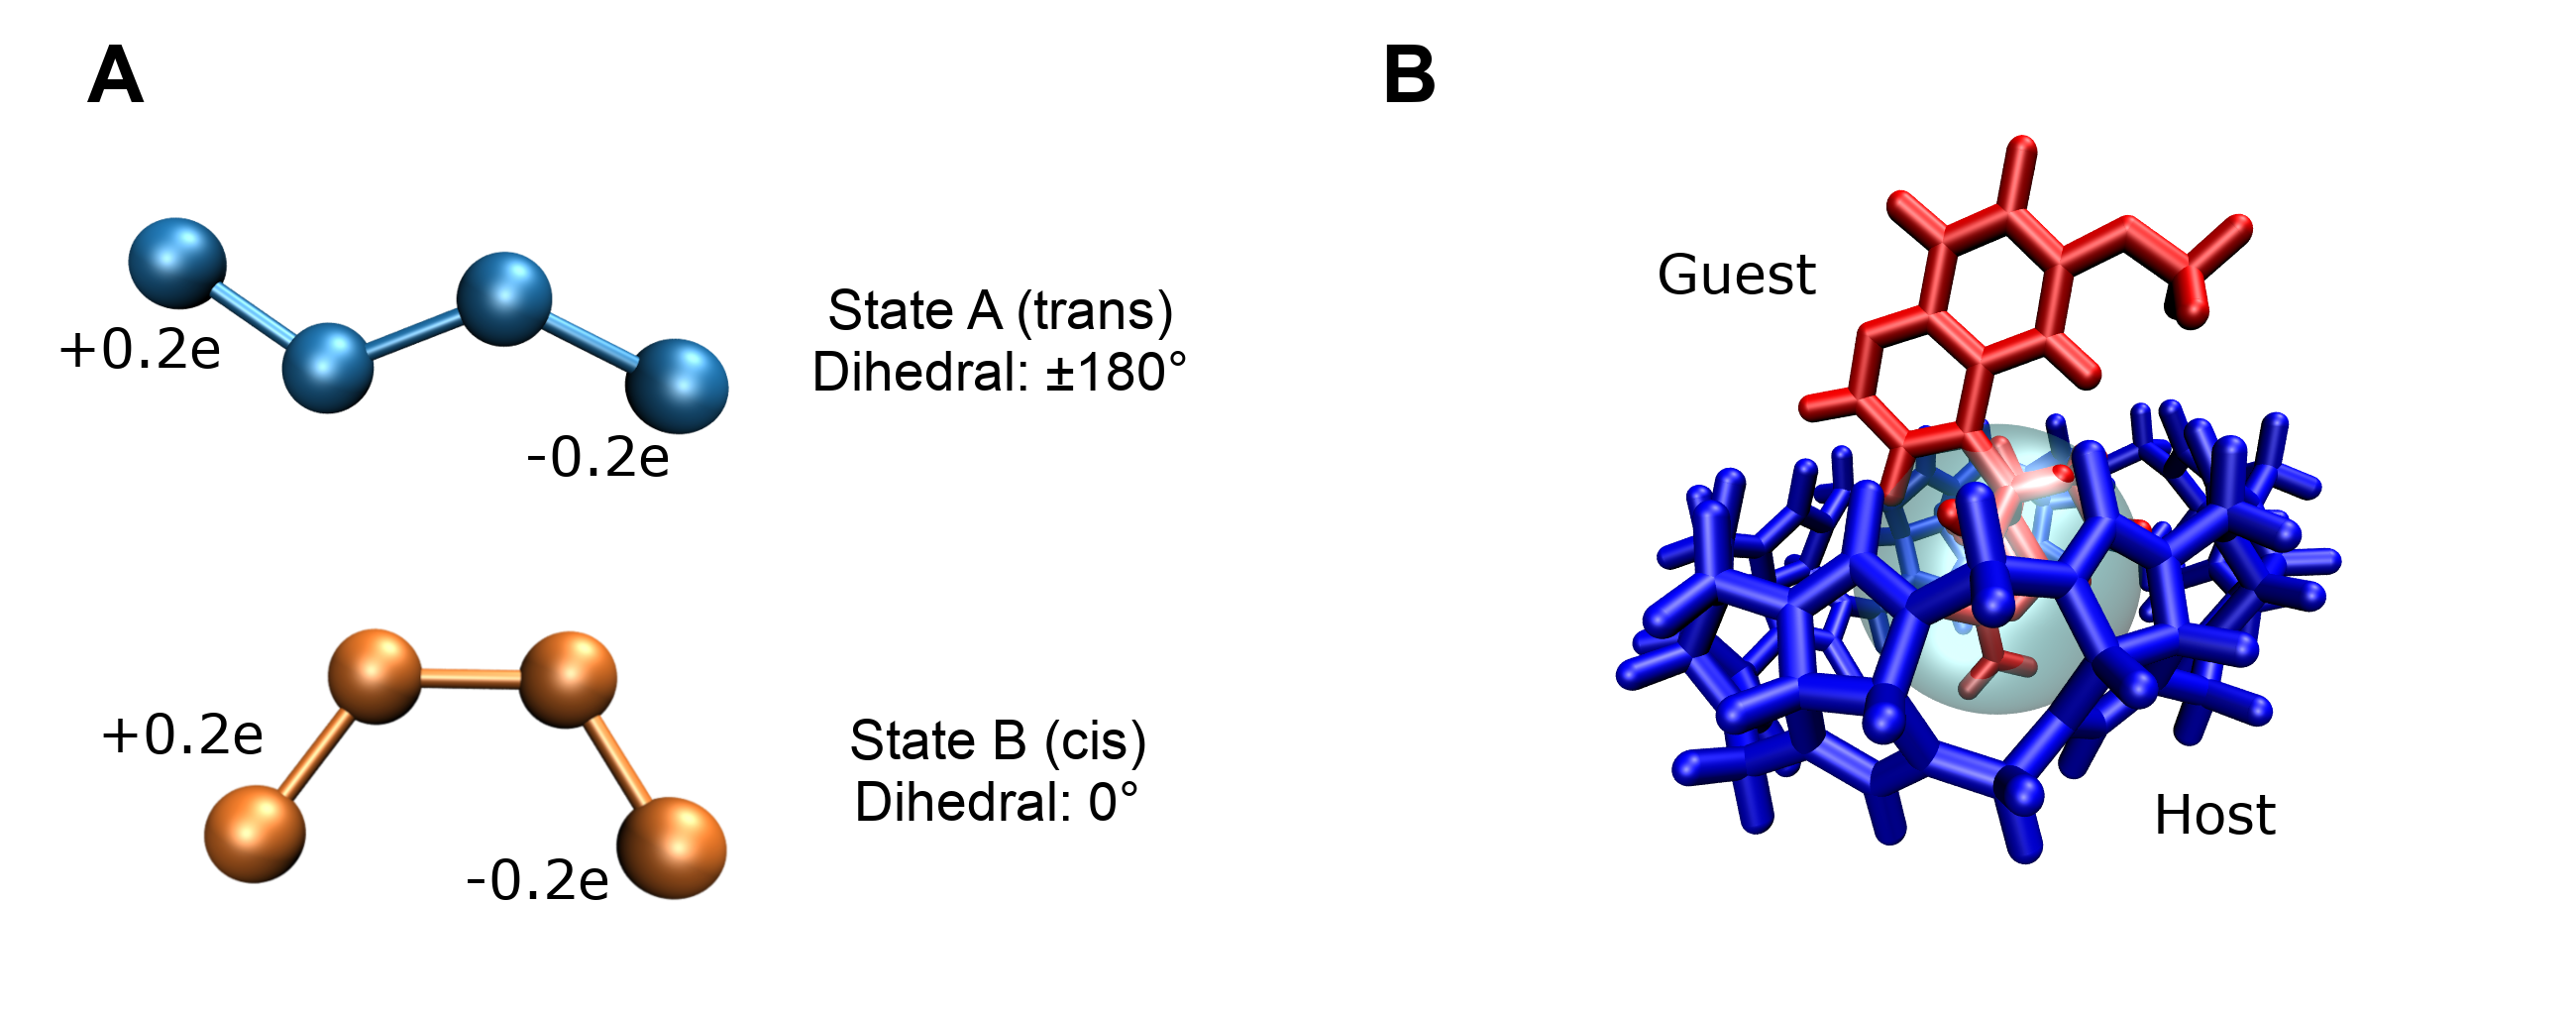
\includegraphics[width=0.9\textwidth]{Figures/sys.png}   
    \caption{(A) The two torsional metastable states of System 2: A molecule composed of 4 interaction sites. The first and last atom have charges of +0.2e and -0.2e, respectively, with the other two atoms uncharged. (B) The bound state of System 3: CB8-G3 host-guest binding complex, with the host molecule (CB8, blue) and guest molecule (G3, red) colored in red and blue, respectively. The fictitious sphere shown in the host molecule was used for estimating the number of water molecules that replace the space of the guest molecule in the binding cavity.}
    \label{test_sys}
\end{figure}

\subsection{System 1: Hydration of an argon atom}
As a sanity check for our implementation of alchemical metadynamics, we used 1D well-tempered alchemical metadynamics to calculate the solvation free energy of an argon atom, which was then compared with the result obtained from an expanded ensemble given the similarity of the two methods. With System 1, the goal is to check if 1D alchemical metadynamics can accurately reproduce the free energy of a simple system calculated by expanded ensemble. 

\subsubsection{Preparation of simulation inputs}
The argon atom was solvated in a cubic box of length 2.4 nm and was energy-minimized by the steepest descent algorithm until the maximum force was lower than 100 kJ/mol/nm. Argon is modeled as a Lennard-Jones sphere with $\epsilon=0.996$ kJ/mol and $\sigma = 0.341$ nm. The system was then equilibrated in the NVT and then NPT ensembles, both for 200 ps. The reference temperature and pressure were maintained at 298 K and 1 bar by the velocity rescaling method~\cite{bussi2007canonical} and a Berendsen barostat~\cite{berendsen1984molecular}, respectively. Lastly, 5 ns of NPT MD simulation with Parrinello-Rahman barostat~\cite{parrinello1980crystal,parrinello1981polymorphic} keeping the pressure at 1 bar was performed, in which the cutoff distance for van der Waals interactions was specified as 0.9 nm. The PME (particle mesh Ewald) method~\cite{essmann1995smooth} was used with a switching function between 0.89 nm and 0.9 nm for efficient calculations of long-range electrostatic interactions. A spacing of 0.10 nm was used for the PME grids. The LINCS~\cite{hess1997lincs} algorithm was used to constrain bonds involving hydrogens, with the highest order in the expansion of the constraint coupling matrix set as 12 and the number of iterative corrections set as 2. The structure whose box volume was the closest to the average volume of the MD trajectory was extracted to serve as the input configuration for the expanded ensemble and alchemical metadynamics simulations, which were both performed in an NVT ensemble to avoid any potential issues with $\lambda$ dependence of pressure. Although this could lead to a slightly different estimate of the solvation free energy as compared to the one solved in the NPT ensemble, the objective is simply to compare two methods with the same alchemical processes in the same ensemble. 

\subsubsection{Expanded ensemble simulation}
We divided our expanded ensemble calculations into two separate stages: an equilibration and a production stage. Both stages of simulations were performed in the NVT ensemble with 6 states for decoupling the van der Waals interactions between the argon atom and the water molecules. In the equilibration stage, we employed the Wang-Landau algorithm to adaptively estimate the weight for each alchemical state, with the initial Wang-Landau incrementor set as 0.5 $\text{k}_{\text{B}}\text{T}$. The histogram that kept track of the state visitation was updated using the Metropolized-Gibbs Monte Carlo moves between all alchemical states every 10 integration steps. We adopted the default value of 0.8 for the cutoff for the flatness ratio $R$, which means that the histogram was considered flat only if all intermediate states had an $R$ value and its reciprocal larger than 0.8. ($R$ is defined as the ratio between the count of a state and the average count of all states.) Whenever the histogram was considered flat, the state counts were all reset to 0 and the Wang-Landau incrementor was scaled by a factor of 0.8. This process for updating weights was stopped when the incrementor fell below 0.001 $\text{k}_{\text{B}}\text{T}$. The equilibrated weights were then used as the frozen weights in the production simulation for 100 ns. For data analysis, we only considered the time series of the Hamiltonian derivative obtained from the production stage. After truncating the non-equilibrium regime~\cite{chodera2016simple} and decorrelating the time series, we ran MBAR~\cite{shirts2008statistically} to compute the free energy difference between the coupled and uncoupled states, which is the solvation free energy of the system. 

\subsubsection{1D alchemical metadynamics}
To compare with expanded ensemble, we adopted the same simulation length (100 ns), starting configuration, state transition scheme (Metropolized-Gibbs sampling), and coupling parameters of the same 6 states in 1D alchemical metadynamics. We set the initial height of the Gaussian biasing potential as 0.5 $\text{k}_{\text{B}}\text{T}$, which is the same as the initial Wang-Landau incrementor despite different weight updating schemes. While in alchemical metadynamics, the strides for Gaussian depositions and MC moves are decoupled and do not need to be the same, we set both strides as 10 integration steps to better compare with expanded ensemble, where a weight is always applied when a move is proposed. To accommodate such a fast pace for applying Gaussian biases, we set the bias factor as 50 to avoid an excessively fast decay in the Gaussian height, which could potentially slow down the compensation of the underlying free energy surface. The width of the Gaussian was set as 0.01 to avoid any overlap between the Gaussians deposited at different $\lambda$ values. Note that having such an overlap would not invalidate the method, but might have made the comparison to expanded ensemble less straightforward. For the solvation free energy calculation, we set the truncation fraction and the average fraction as 0.25 and 0.75, respectively. 1000 blocks were used in the histogram construction, which led to a block size of 75 ps and the largest uncertainty among the considered numbers of blocks in the estimation of the solvation free energy. 200 bootstrap iterations were used in block bootstrapping. 

\subsection{System 2: A 4-site system}
To demonstrate the advantages of introducing configurational CVs in alchemical metadynamics, we designed a fictitious molecule composed of 4 linearly bonded interaction sites as the second system (see Figure \ref{test_sys}A). We placed opposite charges on the first and last atoms (+0.2e and -0.2e) and set the force constant for the only torsional angle as 60 kJ/mol so that the two torsional metastable states of the system were separated by a large free energy barrier (around 48.5 $\text{k}_{\text{B}}\text{T}$, see Figure S3A). Such a large free energy barrier poses a challenge of sampling both torsional metastable states to alchemical free energy methods that do not apply any configurational bias, such as expanded ensemble or 1D alchemical metadynamics. Such a challenge is useful for us to highlight the difference between methods with or without the application of configurational biases in free energy calculations. With this system, we performed a 1D and 2D well-tempered alchemical metadynamics starting from either metastable state to calculate the solvation free energy of the system. The goal is to show that 2D alchemical metadynamics starting from different torsional metastable states leads to statistically consistent estimates of the solvation free energy, which cannot be accomplished by 1D alchemical metadynamics due to restricted configurational sampling. 

\subsubsection{Preparation of simulation inputs}
After solvating System 2 in a dodecahedral box with 1 nm between the solute and box edges, we processed the system with the same procedure of solvation, energy minimization, NVT and NPT equilibration, and NPT MD simulation like the one used in System 1. A structure that had a volume closest to the average over the NPT volume was taken as the input of a 5 ns NVT metadynamics that only biased the torsional angle of the system. This torsional metadynamics applied a Gaussian biasing potential every 500 integration steps, with a bias factor of 10. The width and initial height of the Gaussians were set as 0.5 rad and 1 $\text{k}_{\text{B}}\text{T}$, respectively. With this setup, the system was able to sample both torsional metastable states frequently in the torsional metadynamics (see Figure S3B), from which we generated the structures corresponding to the trans isomer (State A) and cis isomer (State B) for starting subsequent alchemical metadynamics elaborated in later sections. 

\subsubsection{Alchemical metadynamics}
For each torsional metastable state of the system, we started a 1D and 2D well-tempered alchemical metadynamics in an NVT ensemble, where the only torsional angle of the system was introduced in the latter as the second CV. The MC moves between alchemical states were proposed every 10 integration steps using the Metropolized-Gibbs MC scheme. All four simulations were performed for 200 ns and adopted a deposition stride of 500 steps. 20 alchemical intermediate states were used to decouple the van der Waals interactions and Coulombic interactions. 1D alchemical metadynamics started with a Gaussian height of 1 $\text{k}_{\text{B}}\text{T}$, with the bias factor set as 60, while 2D alchemical metadynamics utilized a Gaussian height of 2 $\text{k}_{\text{B}}\text{T}$, and a bias factor of 120 for flattening a much larger phase space. The widths of the Gaussian along the alchemical direction (for 1D and 2D simulations) were set as 0.001, while the Gaussian width in the torsional dimension (for the 2D simulations) was set as 0.5 rad. For all four simulations, we specified a truncation fraction of 0.25 and an average fraction of 0.75. 1000 blocks with a block size of 150 ps were used for all simulations, except for the 1D alchemical metadynamics starting from state A, which used 2000 blocks for histogramming in free energy calculations. 200 bootstrap iterations were used in block bootstrapping. 

\subsection{System 3: CB8-G3 host-guest binding complex}
To further exemplify the usage of alchemical metadynamics, we considered the CB8-G3 host-guest binding complex (see Figure \ref{test_sys}B) as the third test system, which is composed of a cucurbit[8]uril (CB8, host) and a quinine (G3, guest) and is one of the binding complexes in SAMPL6 SAMPLing challenge~\cite{rizzi2018overview}. The binding free energy calculation of this system is considered particularly challenging due to the long time scale of the water motion, especially the exclusion of water molecules from the binding cavity during the binding event (the so-called water-exclusion problem)~\cite{rizzi2020sampl6}. The past literature~\cite{rizzi2020sampl6} shows that expanded ensemble was not able to equilibrate the Wang-Landau weights within the same time used for other binding complexes in the same challenge. Methods such as OpenMM/SOMD and NAMD/BAR replicate calculations could not converge the average free energy to uncertainties under 1 kcal/mol. OpenMM/HREX and AMBER/APR could reach sub-kcal/mol uncertainties, but both of them displayed a significant and slowly decaying bias, requiring a very long time to converge the free energy. Here, our goal is to compare 2D alchemical metadynamics with its 1D analog to show its superiority in accelerating the water motion and accurate estimation of the binding free energy of the binding complex. 

\subsubsection{Preparation of simulation inputs}
We started from the initial files provided by SAMPL6 SAMPLing challenge, which included the coordinates and topology files of the solvated binding complex and the solvated ligand alone. We re-equilibrated both systems in an NPT MD simulation with the same settings as used in Systems 1 and 2. We then extracted the configurations corresponding to the average NPT volumes as the input structures of later simulations.  

\subsubsection{The double decoupling scheme for the binding free energy calculation}
We used the double decoupling method~\cite{gilson1997statistical} with the thermodynamic cycle shown in Figure \ref{thermo_cycle} to decompose the binding free energy calculation of CB8-G3 binding complex. Starting from state A, we split the binding event into two alchemical processes (from A to B and from C to D) bridged by the transfer of the ligand molecule into the binding cavity of the host molecule (from B to C). The first alchemical process (from A to B) decoupled the ligand from its surroundings and was termed as the solvent simulation. The second alchemical process (from C to D) was characterized in the complex simulation, where we started from state D and gradually turn off the non-bonded interactions between the host and guest molecules to calculate $-\Delta A^{\text{solv}}_{\text{(elec + vdW)}_{\text{off}}}$ rather than $\Delta A^{\text{solv}}_{\text{(elec + vdW)}_{\text{off}}}$. Frequently, in the complex simulation, a harmonic restraint is applied between the host and guest molecules to prevent the guest molecule from drifting away and slowing down the convergence. However, the periodic boundary conditions may be easily broken by a known bug in the pull code working with expanded ensemble, so we did not apply any restraint in the system but assumed that the ligand was able to sample to the entire simulation box in the decoupled state. The assumption turned out to be valid (see Figure S1) and allowed us to calculate the box volume correction term $\Delta A_{\text{corr}}$ analytically to bring the affinity in units of the standard concentration. Namely, 
\begin{equation}
    \Delta A^{\circ}_{\text{bind}} = \Delta A_{\text{bind}} + \Delta A_{\text{corr}} = \Delta A_{\text{bind}} - k_{\text{B}}T \ln \left(\frac{V_{\text{box}}}{V_{0}}\right)
\end{equation} where $\Delta A^{\circ}_{\text{bind}}$ is the binding free energy under standard temperature and pressure, $V_{\text{box}}$ is the box volume and $V_0$ is the molecular volume (1.6605 nm$^3$) corresponding to the 1 mol/L reference concentration. 
\begin{figure}[ht]
    \centering
    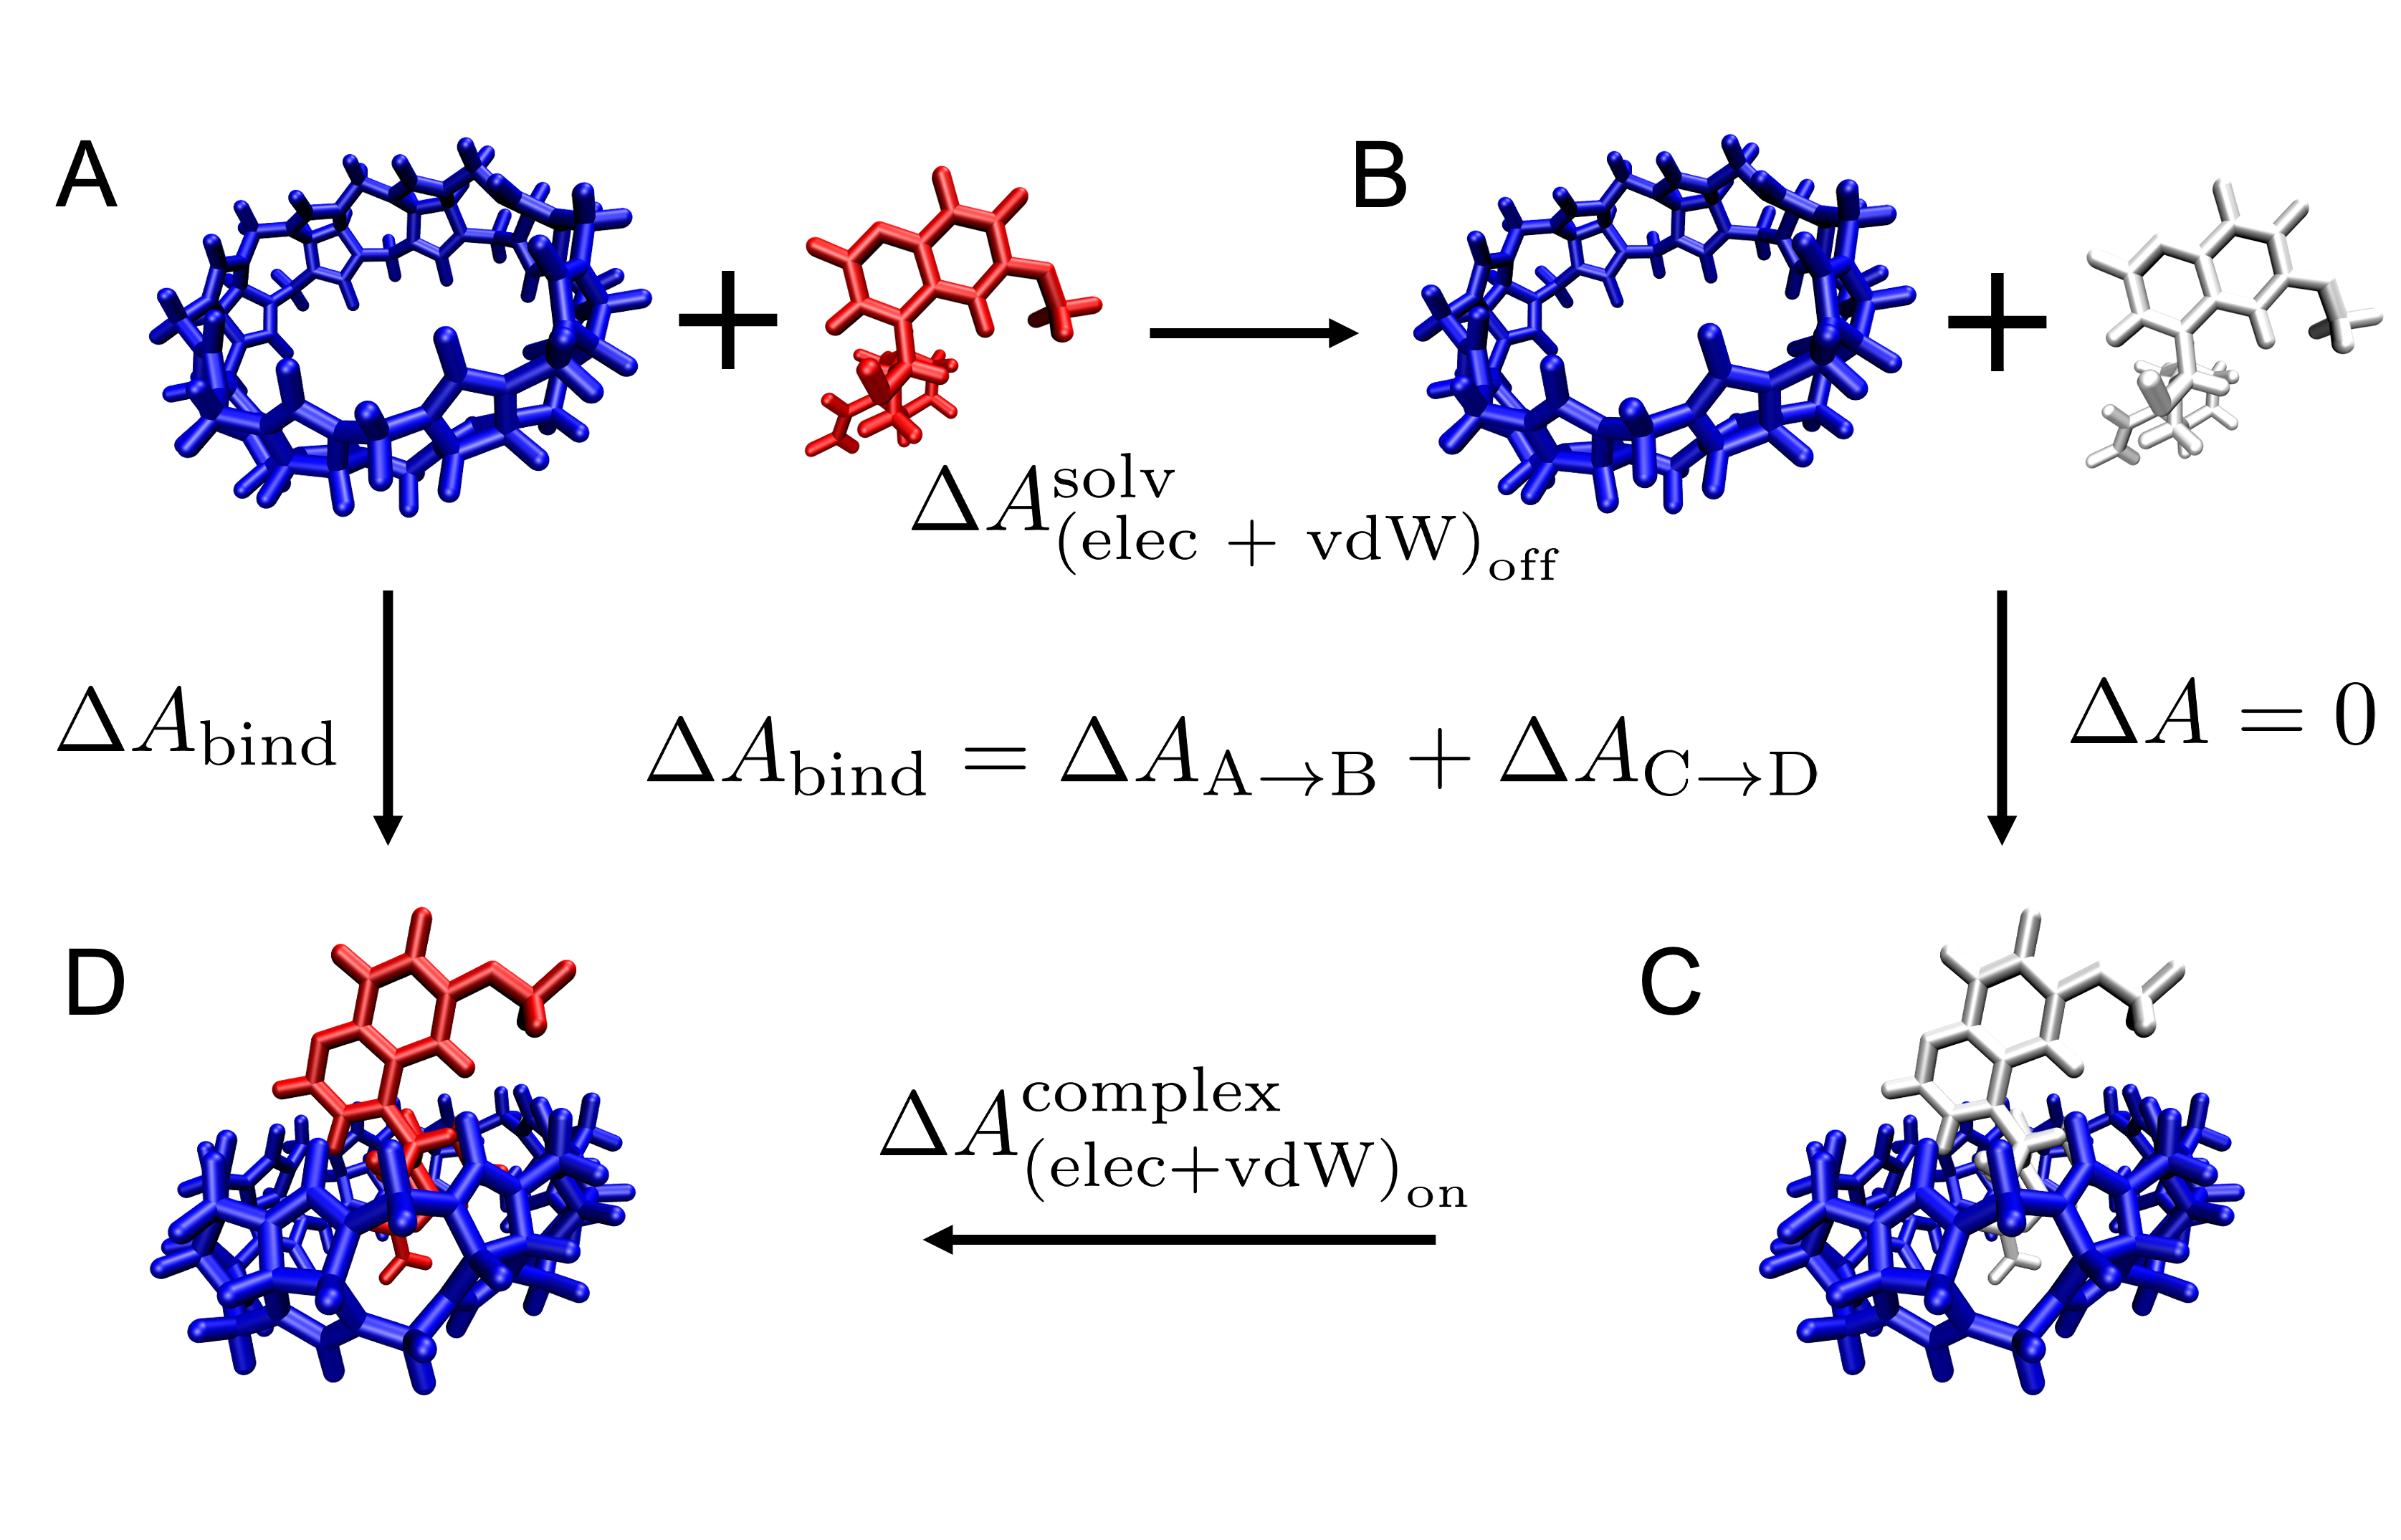
\includegraphics[width=0.8\textwidth]{Figures/cycle_final.png} 
    \caption{The double decoupling thermodynamic cycle for the binding free energy calculation of CB8-G3 host-guest binding complex. The host molecule was colored in blue, while the guest ligand was colored in either white (fully decoupled from the host) or red (fully coupled with the host).}
    \label{thermo_cycle}
\end{figure}

\subsubsection{Alchemical metadynamics}
We used 1D well-tempered alchemical metadynamics in the NVT ensemble as the solvation simulation. 40 alchemical intermediate states were used to gradually decouple the non-bonded interactions between the ligand and the solvent, with Metropolized-Gibbs moves between them attempted every 10 integration steps. Gaussians with a width of 0.01 and the initial height of 2 $\text{k}_{\text{B}}\text{T}$ were deposited with the same frequency as the MC moves, with its decaying rate characterized by a bias factor of 100. We computed $-\Delta A^{\text{solv}}_{\text{(elec + vdW)}_{\text{off}}}$ from 50 block histograms (block size of 1.5 ns) constructed upon the CV time series processed with a truncation fraction of 0.25 and an average fraction of 0.75 for reweighting. 200 bootstrap iterations were carried out in block bootstrapping to estimate the error of the free energy difference. 

For the complex simulation, we performed and compared both 1D and 2D well-tempered alchemical metadynamics in the NVT ensemble. The two simulations utilized the same parameters except the ones in 2D alchemical metadynamics for sampling the additional CV. Specifically, both simulations applied 40 alchemical intermediate states to decouple the non-bonded interactions between the host and guest molecules. The strides for MC moves and Gaussian depositions were both 10 integration steps. The Gaussian biasing potentials had a width of 0.01 and the initial height of 5 $\text{k}_{\text{B}}\text{T}$. The bias factor was set as 150 to overcome the significant probability imbalance between the coupled and uncoupled states. Note that this is common in both the solvent and complex simulations and it necessitated the relatively frequent deposition of the biasing potentials. 

In 2D alchemical metadynamics, the number of water molecules $N$ in the binding cavity that replaced the space of the guest molecule was introduced as the additional configurational CV. The value of $N$ was estimated as the coordination number $S$ between any host atom (set A) and any oxygen atom of the water molecules (set B) in the fictitious sphere shown in Figure \ref{test_sys}B. The sphere was centered at the COM of the host molecule and had a radius of $R_0=0.35$ nm. Mathematically, this is done by a switching function (see Figure S4) to ensure continuous derivatives:
\begin{equation}
    S = \sum_{i\in A}\sum_{j\in B}\frac{1}{1+\left(\frac{r_{ij}}{R_0}\right)^{6}}
\end{equation} where $r_{ij}$ is the inter-particle distance between atoms in sets $A$ and $B$. Note that we did not aim to exclude all the water molecules because the bound state of the binding complex could still have water molecules in the binding cavity. To avoid wasting time in configurations that were likely to be unphysical, we set an upper and lower harmonic wall potential (with the force constant equal to 200 kJ/mol) at $N=10.5$ and $N=0.7$, respectively. These cutoffs were decided from the time series obtained from 10 standard MD simulations of the binding complex (see the section of Standard MD simulations of System 3 in the SI). All the standard MD simulations were performed in an NVT ensemble for 200 ns and utilized the same protocol and parameters as the ones used in the NVT equilibration during the preparation of Systems 1 or 2. 

For the calculation of the free energy difference $\Delta A^{\text{complex}}_{\text{(elec+vdW)}_{\text{on}}}$, we adopted a truncation fraction of 0.25 and an average fraction of 0.75 for both 1D and 2D alchemical metadynamics. 100 blocks (block size: 1.5 ns) and 50 blocks (block size: 3 ns) were respectively used in the two cases for data histogramming, which was followed by 200 bootstrap iterations in block bootstrapping. While the protocol for data analysis of the 1D simulation was not different from the one previously described, for the 2D alchemical metadynamics, we defined the unbiasing weight for each sample differently as 
\begin{equation}
    w(\bfv{\xi'}) = \exp\left(\frac{\bar{V}_{\text{tot}}(\bfv{\xi'}, t_0)}{k_{\text{B}}T}\right)
\end{equation} where $\bar{V}_{\text{tot}}(\bfv{\xi'}, t_0)=\bar{V}(\bfv{\xi'}, t_0) + V_{\text{walls}}(N)$ is the total bias that includes the biases from metadynamics and the sum of both wall potentials ($V_{\text{walls}}$). Such unbiasing weights could remove the influence coming from the wall potentials during the reweighting. With the free energy difference calculated for each alchemical process, we calculate $\Delta A^{\circ}_{\text{bind}}$ by simply summing them up, along with the correction term $\Delta A_{\text{corr}}$. 

\section{Results and discussion}
\subsection{System 1: An argon atom}
With the weights fixed at the values equilibrated by the Wang-Landau algorithm, the solvation free energy of System 1 estimated by expanded ensemble with MBAR was -3.302 $\text{k}_{\text{B}}\text{T}$, with an uncertainty as small as 0.027 $\text{k}_{\text{B}}\text{T}$ owing to sufficiently even state visitation (see Figure S5A). This estimation is statistically consistent with the one obtained from the 1D alchemical metadynamics, which was -3.296 $\pm$ 0.017 $\text{k}_{\text{B}}\text{T}$. Notably, the essential difference in the weight updating approaches between the two methods makes it infeasible to directly compare the performance of the methods. In expanded ensemble, the incrementor decreases in a step-wise manner and the same value is applied to all intermediate states. On the other hand, the Gaussian height in well-tempered metadynamics continuously decays with the amount of biases that have been deposited in the state being sampled, which means that the potential energies of different states are elevated with different amounts depending on how frequently the states have been visited. In our case, the state visitation of expanded ensemble could have been more even if we had adopted a stricter, rather than a typical criterion for histogram flatness, which could also lead to an even smaller uncertainty. With the chosen parameters in our case, though, the expanded ensemble still reached a low uncertainty. More importantly, the data collected from the two simulations is sufficient to indicate that 1D alchemical metadynamics free energy calculations yield results that are equivalent within statistical significance to the expanded ensemble results.

\subsection{System 2: A molecule composed of 4 interaction sites}
The purpose of System 2 is to demonstrate the difference in the configurational sampling between alchemical metadynamics with or without the introduction of the configurational bias. As a consequence, in both 1D alchemical metadynamics simulations, the accumulation of one-dimensional alchemical biases allowed the system to freely sample all the intermediate states (see Figure S6). However, such biases did not facilitate the compensation of the free energy wells along the torsional direction. With the lack of direct biases in the torsional direction, the interconversion of the two isomers became the slowest degree of freedom that trapped the system. Accordingly, it can be seen in Figure \ref{dihedral_A_B}A that 1D alchemical metadynamics failed to sample both metastable states regardless of which torsional state the simulation was initialized at. This insufficient sampling of the torsional space caused the dependence of the estimated solvation free energy on the starting torsional metastable state. Specifically, the solvation free energies estimated by 1D alchemical metadynamics starting from State A and State B were 0.707 $\pm$ 0.032 $\text{k}_{\text{B}}\text{T}$ and -0.232 $\pm$ 0.033 $\text{k}_{\text{B}}\text{T}$ (see Figure \ref{sys2_df_results}), respectively. As either simulation 
failed to account for the potential energy contribution of the other metastable state, the free energy estimates were statistically inconsistent with each other. 

\begin{figure}[ht]
    \centering
    \includegraphics[width=\textwidth]{Figures/dihedral_A_B_annotated.png}   
    \caption{The sampled torsional angle in (A) 1D alchemical metadynamics and (B) 2D alchemical metadynamics as a function of time. As can be seen in the figure, the sampling in the torsional space is restricted in 1D alchemical metadynamics, but essentially complete in its 2D analog.}
    \label{dihedral_A_B}
\end{figure}

By contrast, the 2D Gaussian biasing potentials in both 2D alchemical metadynamics simulations flattened out the free energy surface both along the alchemical and torsional directions simultaneously, so both simulations were able to sample the alchemical and torsional space exhaustively (see Figure S7 and Figure \ref{dihedral_A_B}B). This comprehensive and even sampling along all the slow degrees of freedom led to statistically consistent binding free energy estimations from State A (0.643 $\pm$ 0.031 $\text{k}_{\text{B}}\text{T}$) and State B (0.697 $\pm$ 0.032 $\text{k}_{\text{B}}\text{T}$), as shown in Figure \ref{sys2_df_results}. In addition, the 2D free energy surface of the system can be accurately recovered from either of the two simulations. Figure \ref{sys2_fes_contour} shows the average of the 2D free energy surfaces obtained from the two 2D alchemical metadynamics simulations and its corresponding contour plot. The difference plot of the two surfaces can be found in Figure S8. From the 2D free energy surface, it is clear that the alchemical variable is orthogonal to the torsional angle of the system, which explains the ineffectiveness of the one-dimensional alchemical bias in the torsional sampling. Notably, this is exactly Scenario A in Figure \ref{EXE_issues} that can fail alchemical free energy methods without the application of configurational biases, so the success in System 2 just verified the usage of 2D alchemical metadynamics in overcoming the extensive free energy barrier present in a certain configurational CV direction. 

\begin{figure}[H]
    \centering
    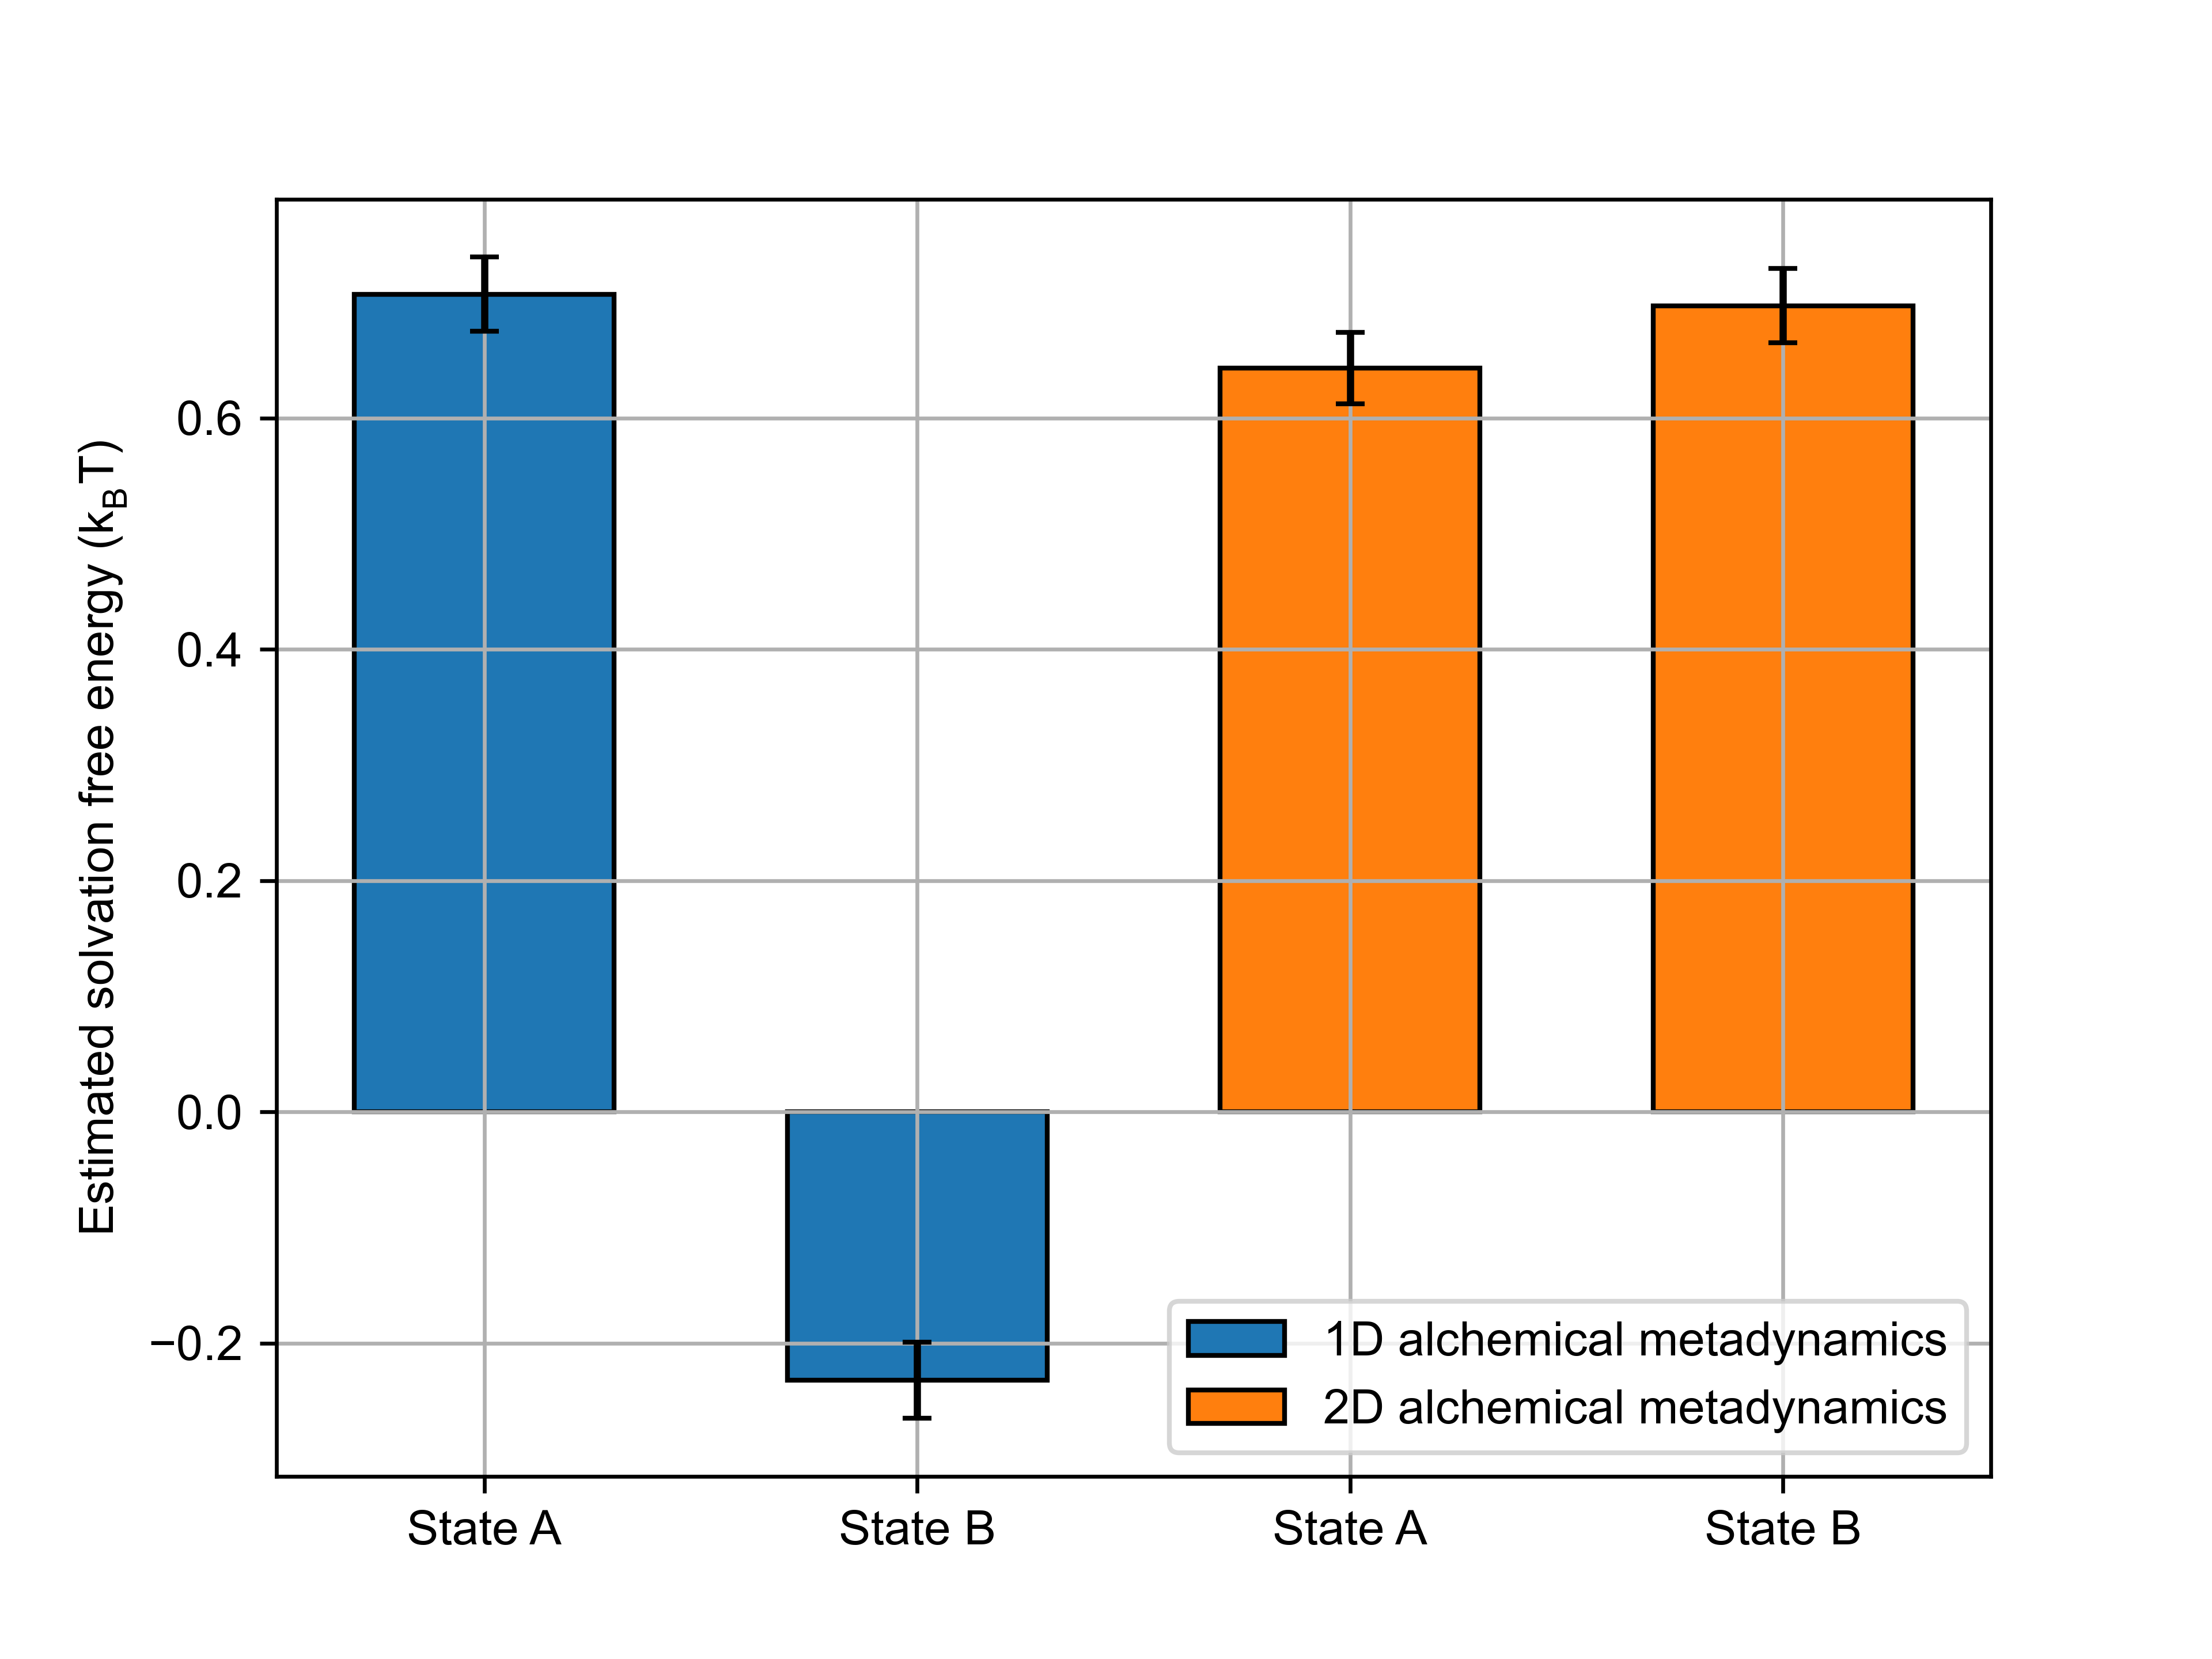
\includegraphics[width=0.7\textwidth]{Figures/sys2_df_results.png}
    \caption{The solvation free energies estimated by 1D and 2D alchemical metadynamics starting from either states. The two 1D alchemical metadynamics simulations starting from different torsional metastable states led to statistically different estimations of the binding free energy, while the values estimated by the 2D simulations are statistically consistent with each other.}
    \label{sys2_df_results}
\end{figure}

\begin{figure}[H]
    \centering
    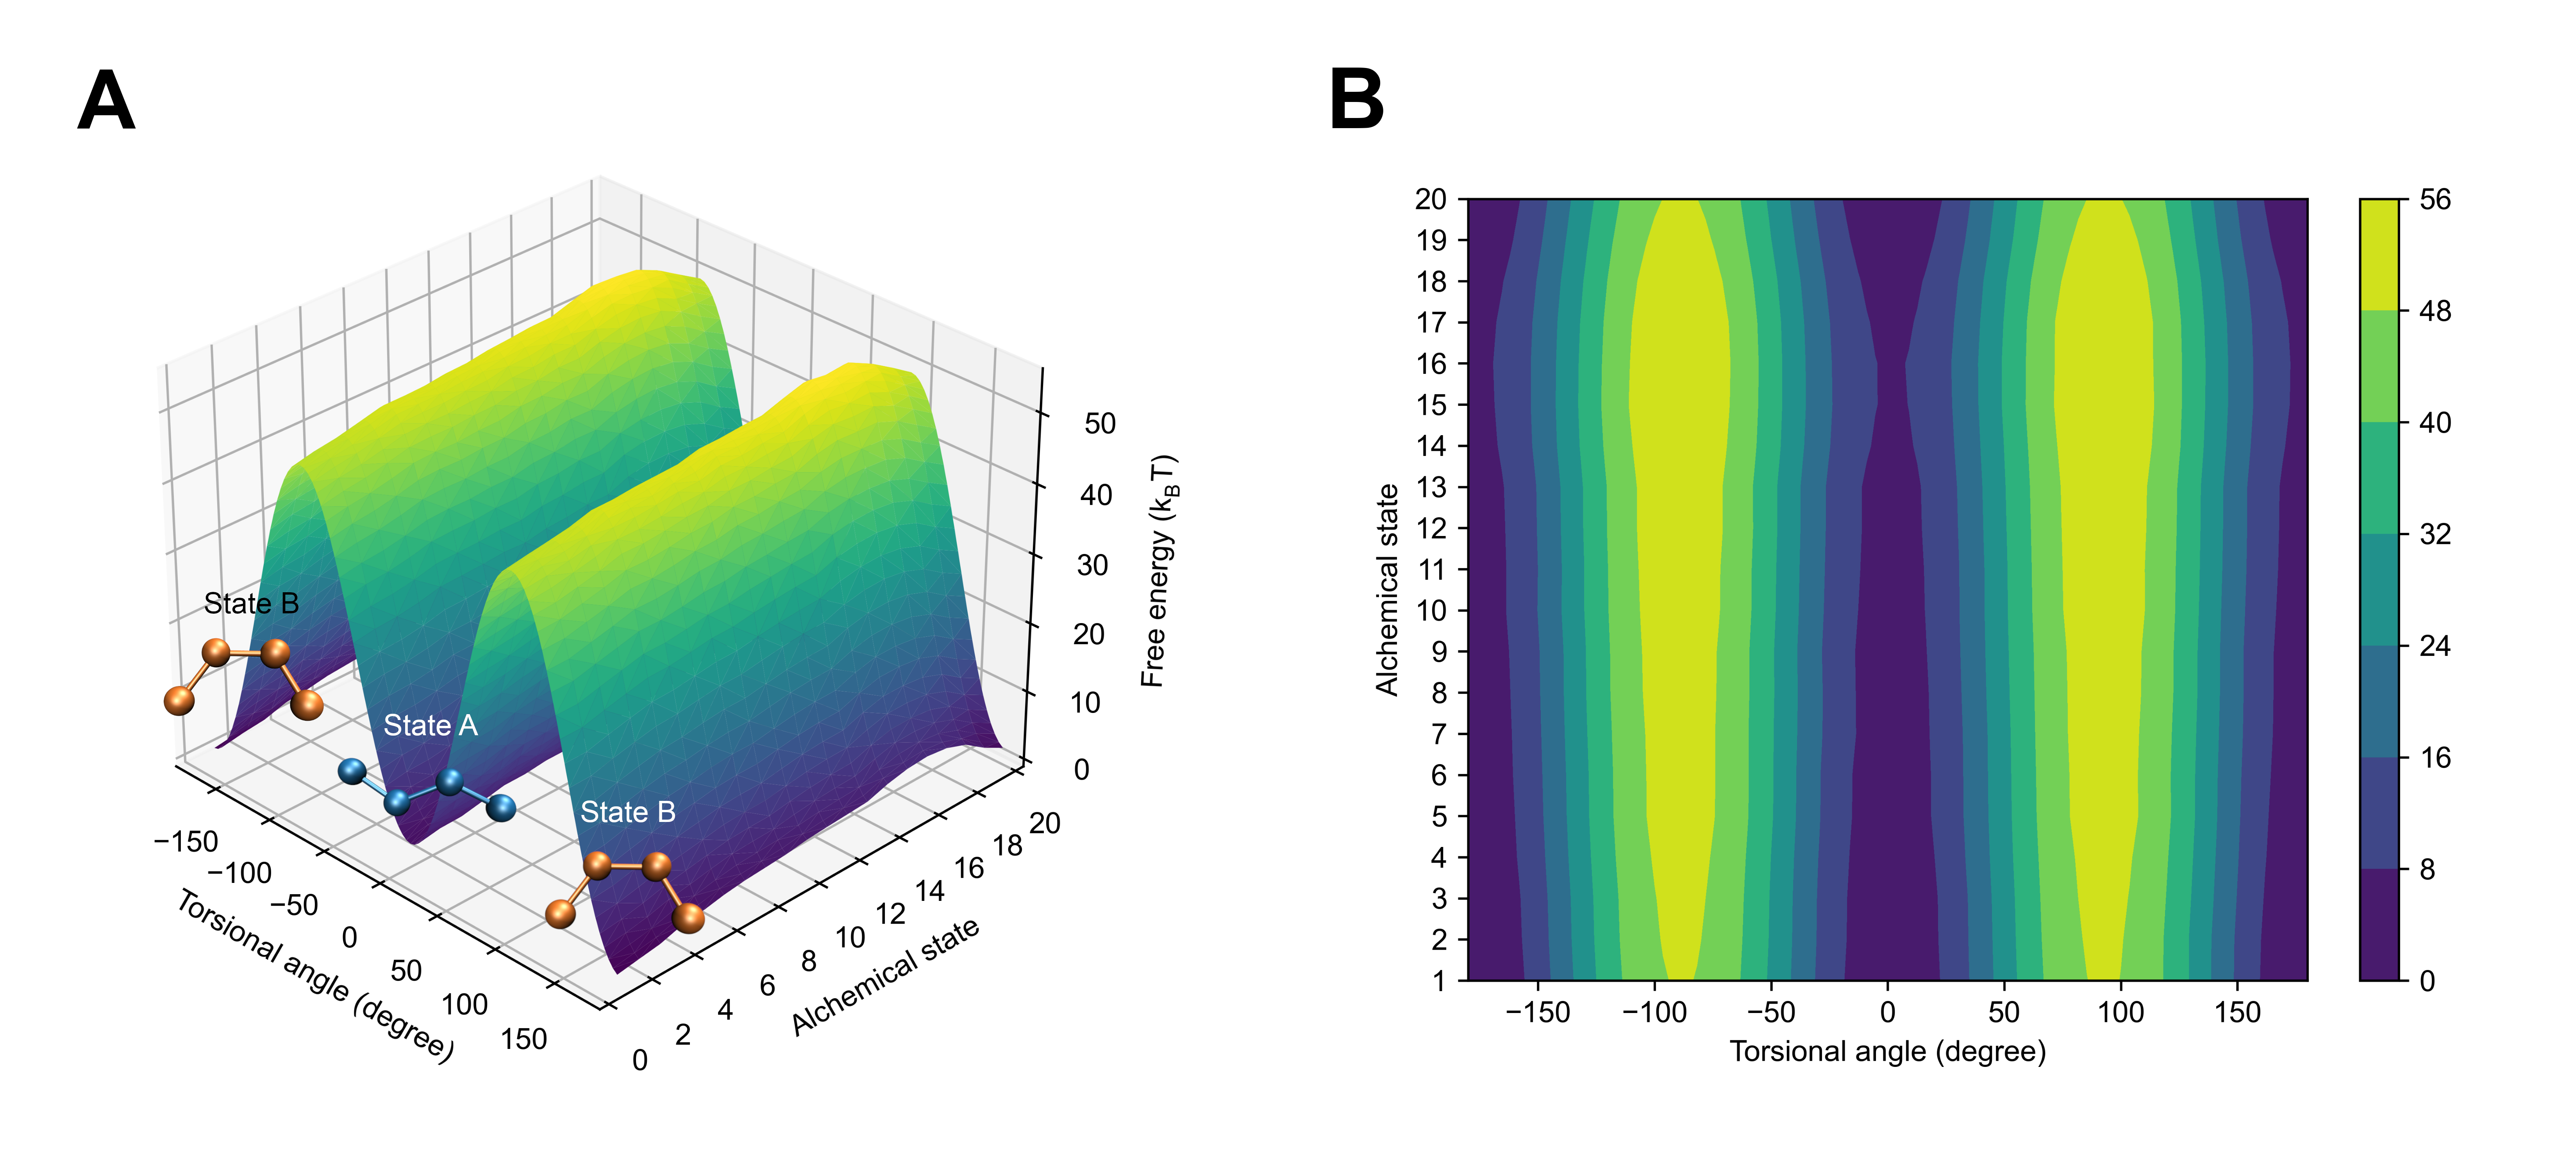
\includegraphics[width=\textwidth]{Figures/sys2_fes_contour_avg_annotated.png}   
    \caption{(A) The average of the 2D free energy surfaces obtained from the two 2D alchemical metadynamics simulations starting from State A and State B. (B) The average of the contour plots obtained from the 2D alchemical metadynamics simulations starting from State A and State B.}
    \label{sys2_fes_contour}
\end{figure}

\subsection{System 3: CB8-G3 host-guest binding complex}
In System 3, the impediment to frequent sampling of both the bound and unbound states is the long time scale of the water molecules entering and exiting the binding cavity. Our hypothesis is that the 2D alchemical metadynamics can accelerate the slow water motion and thus reduce the time needed to converge the sampling. 

To examine how the dynamics of the water molecules was changed upon the introduction of the configurational CV in the complex simulation, we plotted the time series of the number of water molecules in the fictitious sphere (see Figure \ref{test_sys}) representing the volume occupied by the guest ligand (see Figure \ref{water_timerseries}). As a result, in the course of the 200 ns 1D alchemical metadynamics, there were only 3 rounds of binding/unbinding events. More specifically, Figure \ref{water_timerseries}A shows that it only took 2 to 9 ns for the water to enter the binding cavity after the ligand unbound, while the water exclusion always took more than 45 ns. Notably, the alchemical variable is not strictly orthogonal to the number of water molecules, which implies that the alchemical biases could also indirectly bias the motion of the water. This explains the shortened time scale of water inclusion in the 1D alchemical metadynamics as compared to the standard MD simulations of System 3 (see Figure \ref{water_timerseries}A and the section of Standard MD simulations of the binding complex in the SI), as the alchemical biases allowed the system to drift to weakly coupled states where the ligand could unbind easily. This indirect influence from alchemical biases is also evidenced by the several transitions between the two metastable states occurred in the 1D alchemical metadynamics, as contrasted with the lack of transitions in the standard MD simulations of the System 3 (see Figure \ref{water_timerseries}A and the section of Standard MD simulations of System 3 in the SI). It also explains the gradually increasing time scale of the water motion in both directions, which can be ascribed to the fact that decreasing alchemical biases were less efficient in pushing the water molecules into or out of the binding cavity. Unlike the 1D alchemical metadynamics in System 2, the 1D simulation here did sample both configurational metastable states, although the event was too rare to provide reliable statistics in free energy reconstructions, yielding a free energy difference between the coupled and uncoupled states ($-\Delta A^{\text{complex}}_{\text{(elec + vdW)}_{\text{on}}}$) of 133.87 $\pm$ 0.15 $\text{k}_{\text{B}}\text{T}$.

\begin{figure}[ht]
    \centering
    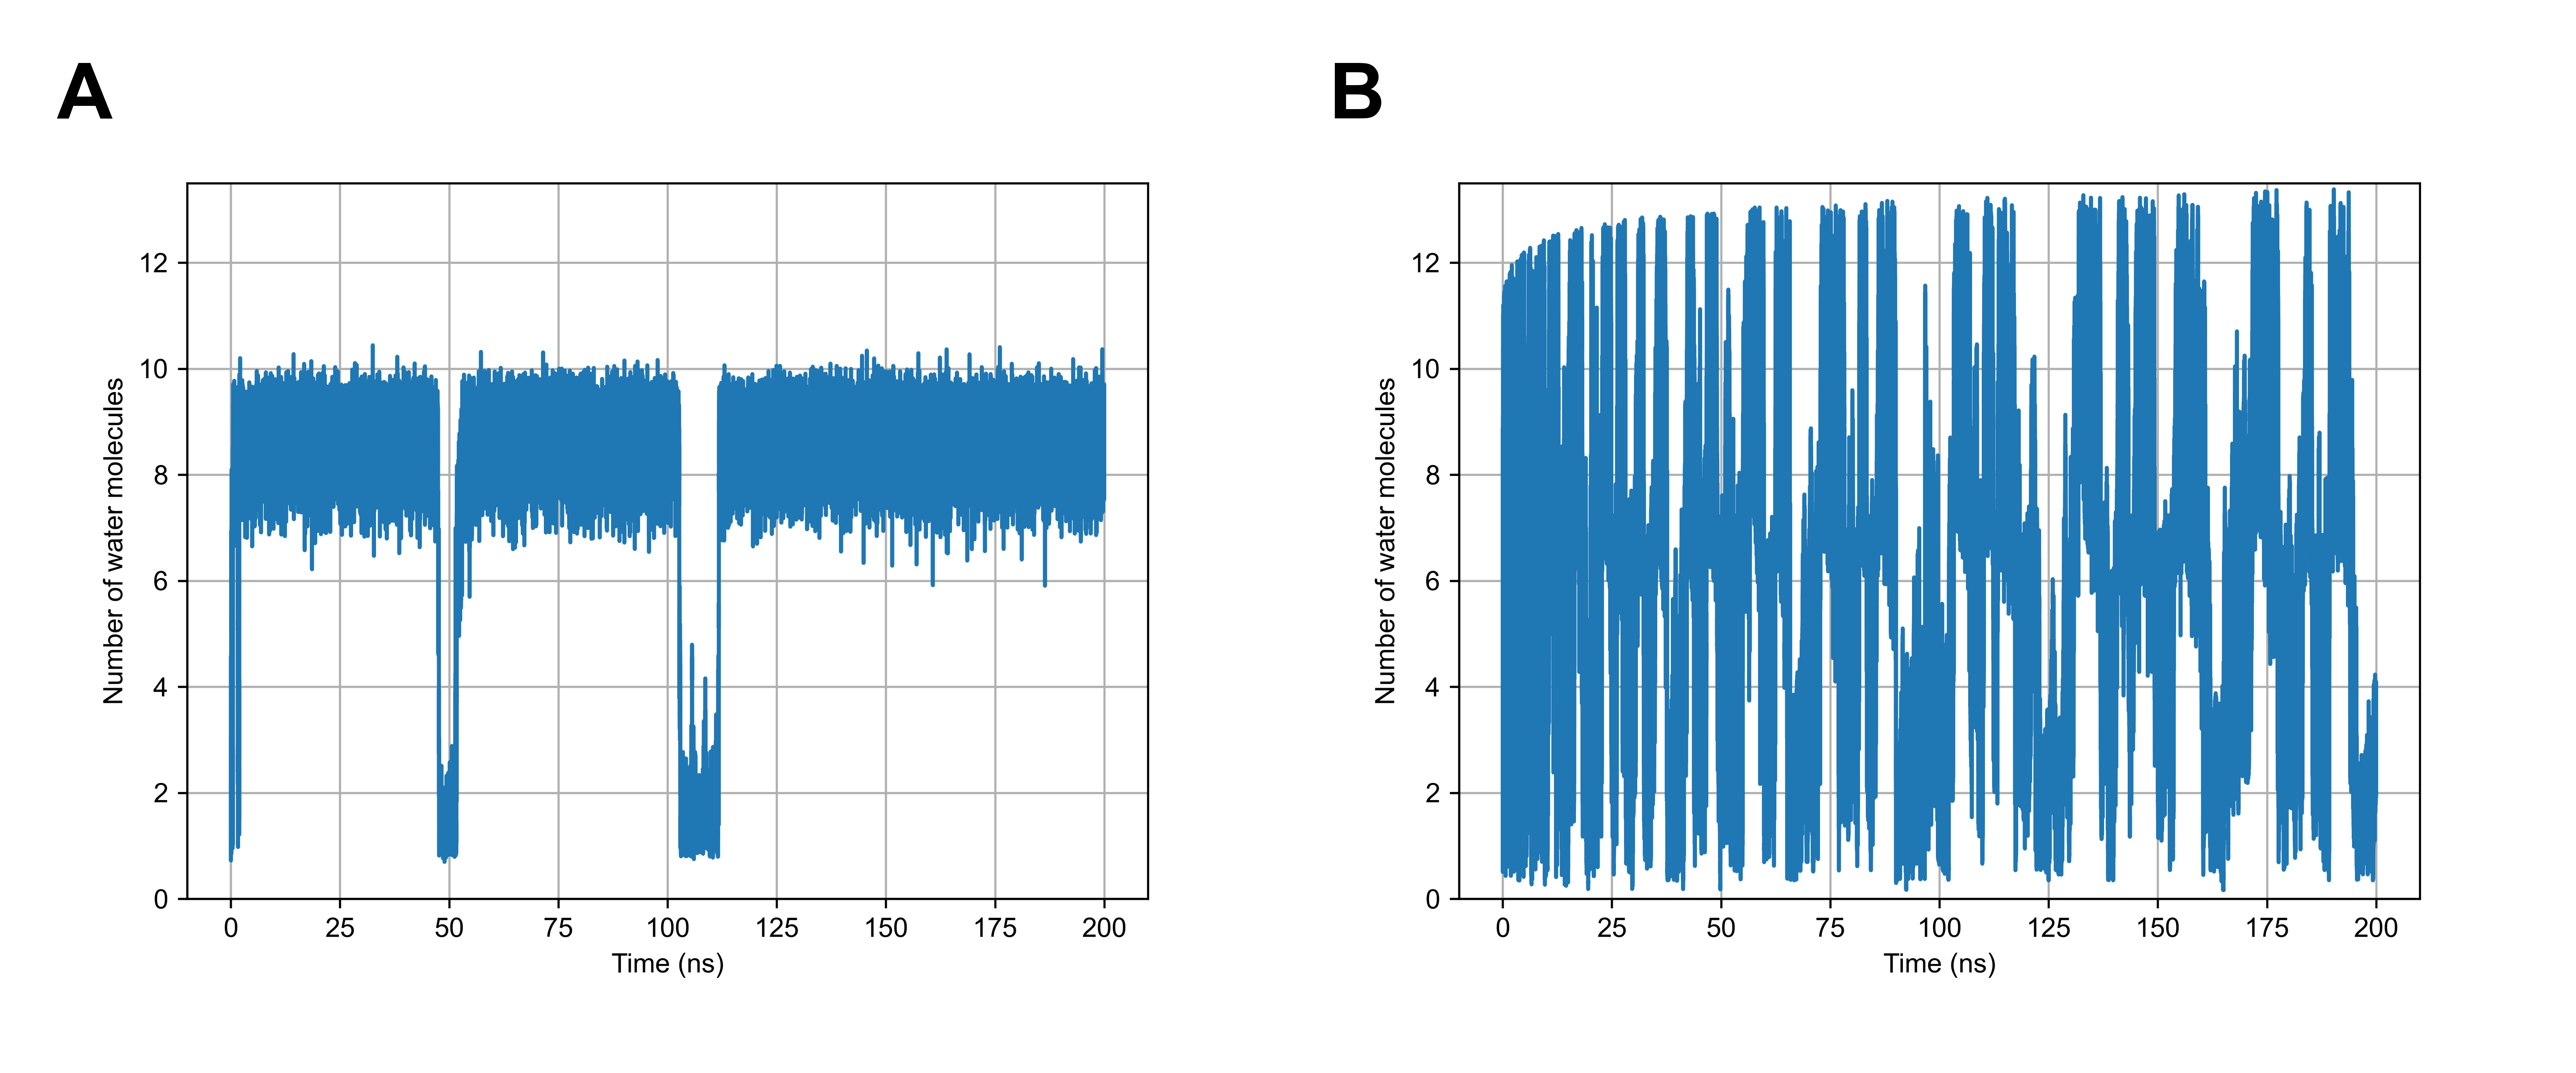
\includegraphics[width=\textwidth]{Figures/water_timeseries.png}  
    \caption{The number of water molecules as a function of time in (A) 1D alchemical metadynamics and (B) 2D alchemical metadynamics. The two figures are using the same scale for the y-axis. As can be seen from the figure, there were much more transitions in 2D alchemical metadynamics compared with the 1D simulation.}
    \label{water_timerseries}
\end{figure}

In the 2D alchemical metadynamics, the acceleration of the water motion no longer merely relied on the marginal contribution from the alchemical bias, but was directly aided by the bias in the configurational direction. As such, the time scale of water exclusion was largely shortened, allowing over 20 transitions between the two metastable states during the simulation. Notably, the water molecules were squeezed in the binding cavity by the configurational bias, so the maximum number of water molecules (13.4) was larger than that in the standard MD simulation (around 10.5) even under the influence of the upper wall potential set at 10.5. Similar to 1D alchemical metadynamics, the time scale of the water motion gradually increased with the decreasing Gaussian height. Given the well-sampled configurational space, the free energy difference between the coupled and uncoupled states ($-\Delta A^{\text{complex}}_{\text{(elec + vdW)}_{\text{on}}}$) was estimated as 132.92 $\pm$ 0.15 $\text{k}_{\text{B}}\text{T}$, which was not far but statistically different from the one obtained in the 1D simulation. 

With the free energy difference $-\Delta A^{\text{complex}}_{\text{(elec + vdW)}_{\text{on}}}$ estimated, we could finally estimate the binding free energy of the binding complex 
$\Delta A^{\circ}_{\text{bind}} = \Delta A^{\text{solv}}_{\text{(elec + vdW)}_{\text{off}}} + \Delta A^{\text{complex}}_{\text{(elec + vdW)}_{\text{on}}} - k_{\text{B}}T \ln \left(\frac{V_{\text{box}}}{V_{0}}\right)$. Specifically, $\Delta A^{\text{solv}}_{\text{(elec + vdW)}_{\text{off}}}$ was estimated to be 131.89 $\pm$ 0.16 $\text{k}_{\text{B}}\text{T}$ by 1D alchemical metadynamics as the solvent simulation, which in theory should be accurate given the comprehensive alchemical sampling (see Figure S9) and the lack of configurational metastable states that the simulation could have missed. The correction term $\Delta A_{\text{corr}}$ was calculated as -3.70 $\text{k}_{\text{B}}\text{T}$, assuming that the guest ligand in the fully decoupled state could sample the entire simulation box, as shown by testing. Consequently, the total binding free energy was estimated to be -4.73 $\pm 0.22$ $\text{k}_{\text{B}}\text{T}$.

Lastly, from the 2D simulation, we additionally recovered the 2D free energy surface of the system, with the dependence between the alchemical variable and the configurational CV removed by shifting the whole free energy surface by its 1D projection along the alchemical direction (see Figure \ref{sys3_2d_fes_contour}). This free energy surface exhibits two high-probability regions in the sampling space, which include the narrow ditch approximately at $N=1$ to $N=1.5$, and a deep basin in higher alchemical states with large $N$ values. The extended ditch clearly corresponds to the bound state, while the deep basin in the weakly coupled states reflects the preference of hydrated configurations over the other end. In the fully coupled state, the free energy barrier peaks around $N=6$, which separates the bound (approximately $N<1.5$) and unbound (approximately $8 < N < 9$). Notably, in the fully coupled state, crossing the free energy barrier from the bound state to the unbound state is harder than in the opposite direction, which caused the extended time scale of water exclusion. On the other hand, water exclusion is the slowest degree of freedom in weakly coupled states that can be reached in alchemical sampling. By flattening out the free energy surface, 2D alchemical metadynamics shortened both time scales. Importantly, the free energy basins shown in Figure \ref{sys3_2d_fes_contour} categorized System 3 as Scenario B in \ref{EXE_issues}, so the escape from such free energy basins demonstrates that alchemical metadynamics that biases configurational CV can address the two most common challenges shown in \ref{EXE_issues} that fail most traditional alchemical free energy methods.

\begin{figure}[ht]
    \centering
    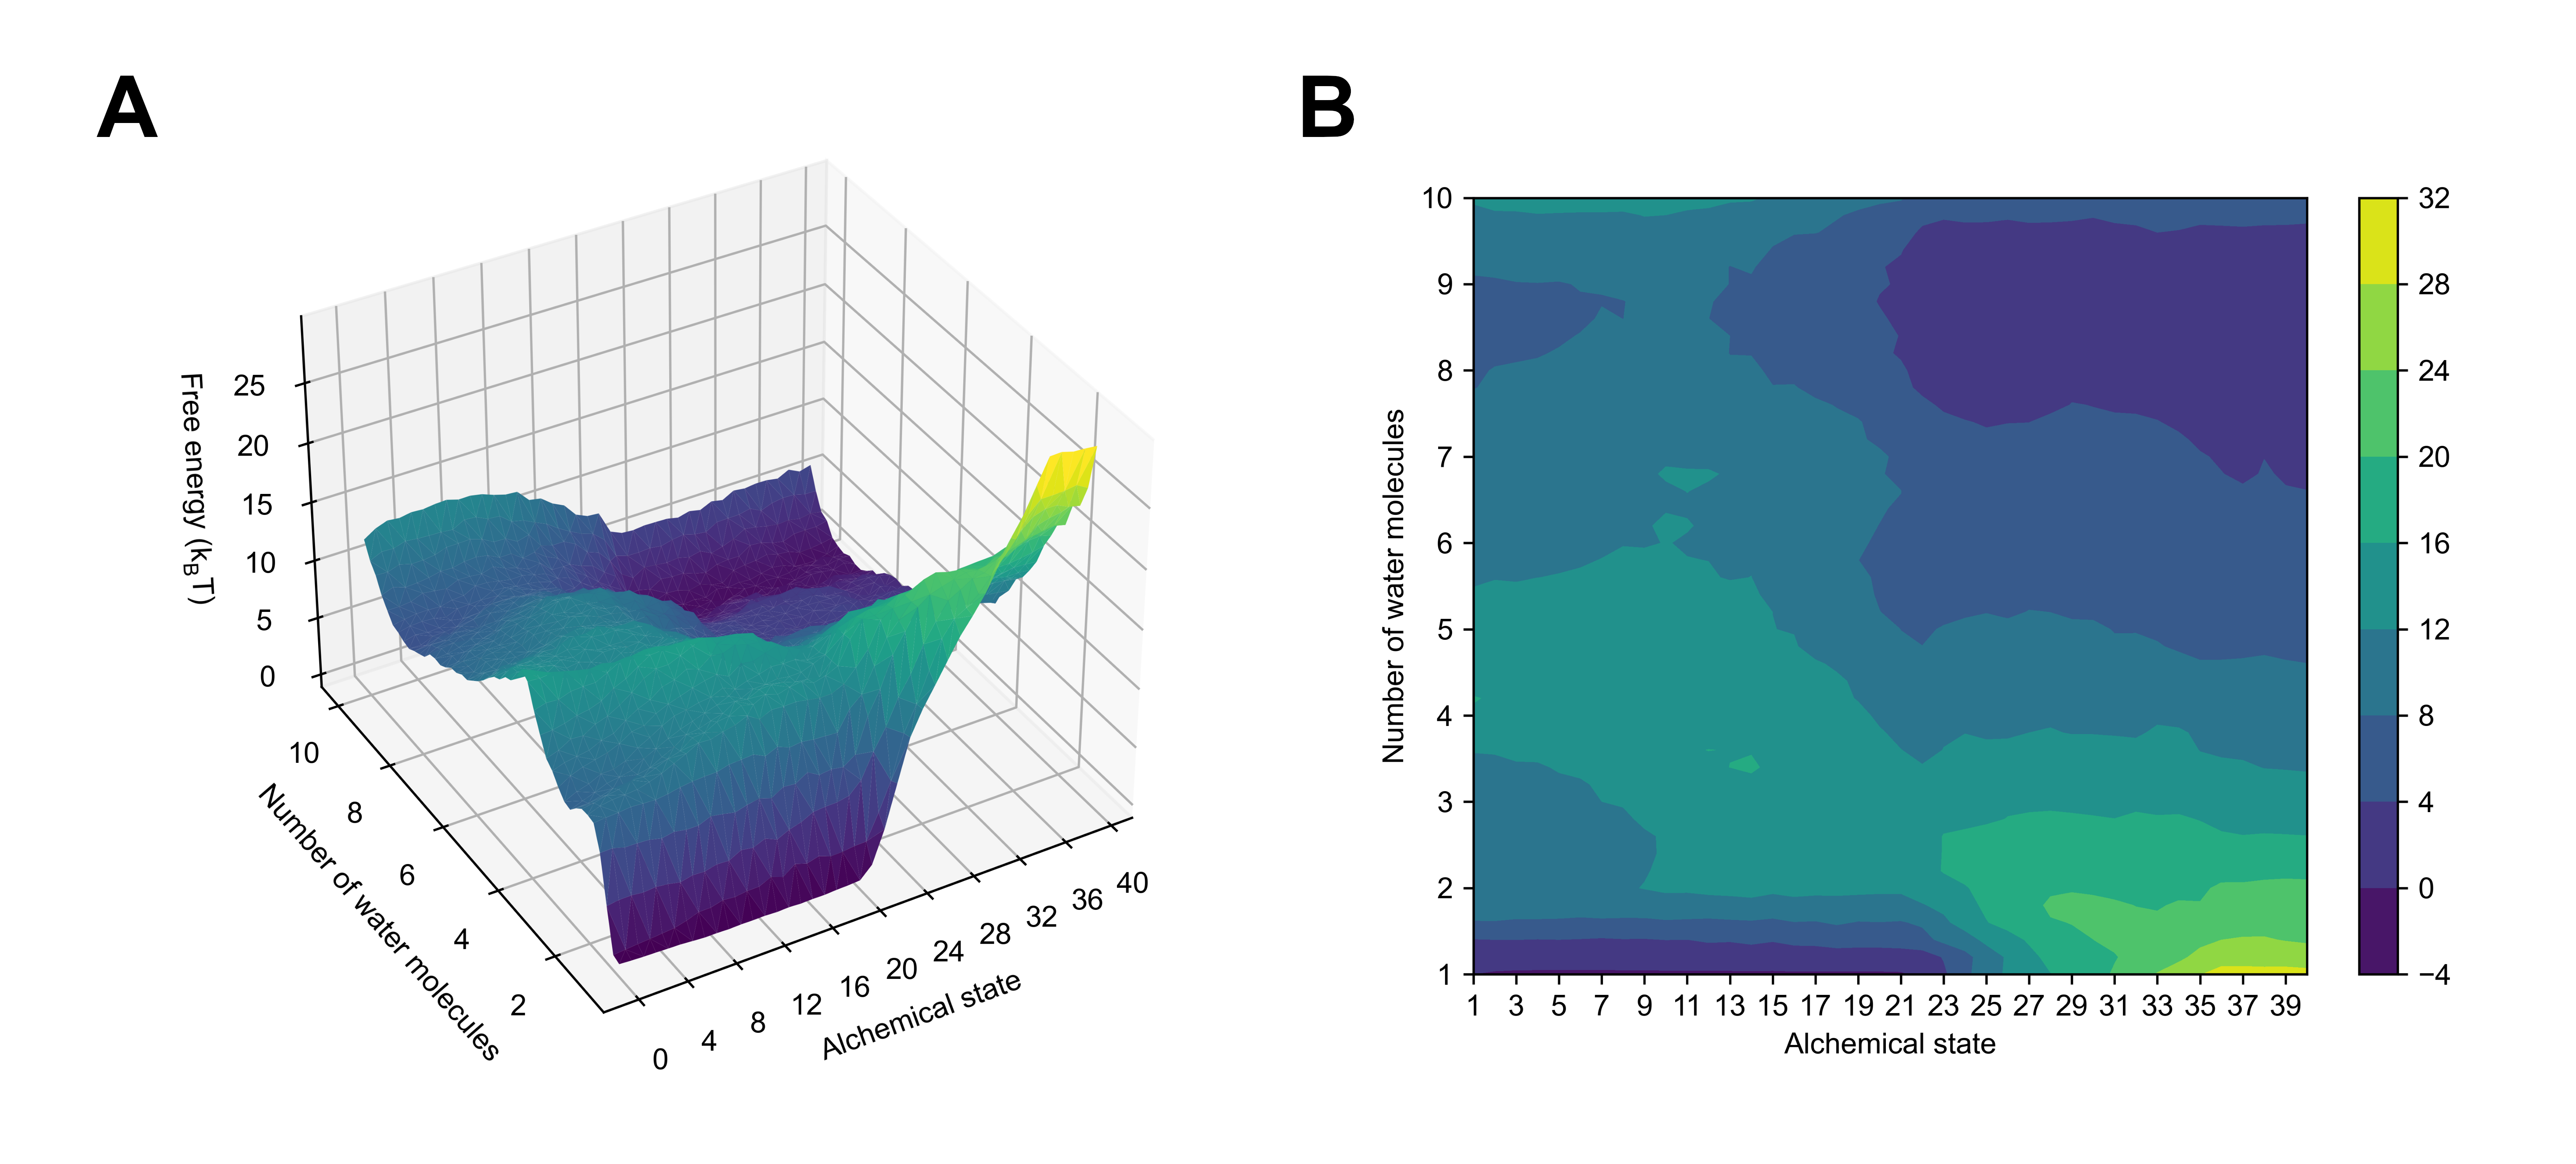
\includegraphics[width=\textwidth]{Figures/sys3_2d_fes_contour_annotated.png}  
    \caption{(A) The 2D free energy surface and (B) contour plot of System 3. The 2D free energy surface was computed from the 2D alchemical metadynamics but the marginalized free energy as a function of $\lambda$ was removed to make it possible to see the free energy in the water occupancy direction as a function of lambda.}
    \label{sys3_2d_fes_contour}
\end{figure}

\section{Conclusion}
In this study, we proposed alchemical metadynamics, which expanded the configurationally defined sampling space allowed in traditional metadynamics with an additional sampling direction. Alchemical metadynamics is most useful when the CV space is multidimensional. With the configurational bias, it encourages the system to escape from configurational metastable subspace that could have easily trap the system. It retains the advantages of traditional alchemical free energy methods, but also enables higher flexibility in sampling rough free energy surfaces. 

With different test systems and alchemical processes, we showed that 1D alchemical metadynamics had at least comparable performance as expanded ensemble, and was able to accurately calculate the solvation free energy of an argon atom. We also showed that 2D alchemical metadynamics could eliminate the dependence of free energy calculations on the starting metastable state due to restricted configurational sampling in System 2. In System 3, we demonstrated that 2D alchemical metadynamics could accelerate the water exclusion by shortening its time scale approximately by a factor of 10. More importantly, the success in both Systems 2 and 3 manifests the usage of alchemical metadynamics in overcoming challenges that can frustrate traditional alchemical free energy methods that do not bias configurational CVs. We conclude that alchemical metadynamics is promising in enhancing sampling in challenging systems, such as highly flexible protein-peptide binding complexes, or protein-nucleic acid binding complexes. The method can be trivially combined with more sophisticated algorithms, such as path collective variable~\cite{branduardi2007b} tICA~\cite{m2017tica}, SGOOP~\cite{tiwary2016spectral}, RAVE~\cite{ribeiro2018reweighted}, or other similar machine learning methods~\cite{rohrdanz2011determination, sultan2018automated, mccarty2017variational, chen2018molecular, wang2019past, wehmeyer2018time}.

\section*{Author Contributions}
W.-T.H., M.R.S. primarily conceptualized the project and designed the methodology, with additional contributions from P.T.M and G.B.; P.T.M. implemented the sampling methods in PLUMED and GROMACS, with contributions from G.B. Experiments were performed by W.-T.H.; experiments were analyzed and validated by W.-T.H. with contributions from M.R.S.; W.-T.H wrote the original manuscript draft; editing and review of the manuscript was done by M.R.S., G.B. and P.T.M. M.R.S. supervised the project and obtained resources.


%%%%%%%%%%%%%%%%%%%%%%%%%%%%%%%%%%%%%%%%%%%%%%%%%%%%%%%%%%%%%%%%%%%%%
%% The "Acknowledgement" section can be given in all manuscript
%% classes.  This should be given within the "acknowledgement"
%% environment, which will make the correct section or running title.
%%%%%%%%%%%%%%%%%%%%%%%%%%%%%%%%%%%%%%%%%%%%%%%%%%%%%%%%%%%%%%%%%%%%%
\begin{acknowledgement}
This study was supported by the grant from National Science Foundation (OAC-1835720) (W.-T.S and M.R.S) and an MolSSI Software Fellowship (P.T.M.). MolSSI is funded by NSF CHE-2136142.  The computational work done in this publication used resources provided from the Extreme Science and Engineering Discovery Environment (XSEDE), which is supported by National Science Foundation grant number ACI-1548562. Specifically, it used the Bridges-2 system, which is supported by NSF  ACI-1928147, located at the Pittsburgh Supercomputing Center (PSC). 

\end{acknowledgement}

%%%%%%%%%%%%%%%%%%%%%%%%%%%%%%%%%%%%%%%%%%%%%%%%%%%%%%%%%%%%%%%%%%%%%
%% The same is true for Supporting Information, which should use the
%% suppinfo environment.
%%%%%%%%%%%%%%%%%%%%%%%%%%%%%%%%%%%%%%%%%%%%%%%%%%%%%%%%%%%%%%%%%%%%%
%\begin{suppinfo}

%\end{suppinfo}

%%%%%%%%%%%%%%%%%%%%%%%%%%%%%%%%%%%%%%%%%%%%%%%%%%%%%%%%%%%%%%%%%%%%%
%% The appropriate \bibliography command should be placed here.
%% Notice that the class file automatically sets \bibliographystyle
%% and also names the section correctly.
%%%%%%%%%%%%%%%%%%%%%%%%%%%%%%%%%%%%%%%%%%%%%%%%%%%%%%%%%%%%%%%%%%%%%
% \clearpage
\bibliography{refs}

\end{document}